
\documentclass[12pt,a4paper]{ctexrep}
\usepackage{amsmath,amssymb}
\usepackage{fontspec}
\xeCJKsetup{AutoFallBack = true}
\setCJKfallbackfamilyfont\CJKrmdefault{Malgun Gothic}[Scale=MatchLowercase]
\setCJKfallbackfamilyfont\CJKsfdefault{Malgun Gothic}[Scale=MatchLowercase]
\setCJKfallbackfamilyfont\CJKttdefault{Malgun Gothic}[Scale=MatchLowercase]
\usepackage[top=1.5cm,bottom=1.5cm,left=1cm,right=1cm,headheight=15pt]{geometry}
\usepackage{pdflscape}

\usepackage{hyperref}
\usepackage{graphicx}
\usepackage{tikz}
\usetikzlibrary{shapes.multipart, shapes.geometric, decorations.pathreplacing, arrows.meta, positioning, matrix, calc}
\usepackage{float}
\usepackage{booktabs}
\usepackage{tabularx}
\usepackage{tabulary}
\usepackage{pgfplots}
\pgfplotsset{compat=1.18}
\usepackage{setspace}
\usepackage{fancyhdr}
\usepackage{algorithm}
\usepackage{algpseudocode}
\usepackage{needspace}
\usepackage{etoolbox}
\usepackage{listings}
\widowpenalty=10000
\clubpenalty=10000
\raggedbottom
\emergencystretch=3em
\tolerance=2000
\setlength{\intextsep}{8pt}
\setlength{\textfloatsep}{10pt}
\pretocmd{\section}{\needspace{13\baselineskip}}{}{}
\pretocmd{\subsection}{\needspace{8\baselineskip}}{}{}
\pretocmd{\subsubsection}{\needspace{5\baselineskip}}{}{}

\lstset{
    basicstyle=\ttfamily\small,
    numbers=left,
    numberstyle=\tiny,
    frame=single,
    breaklines=true,
    showstringspaces=false,
    tabsize=4
}

\onehalfspacing
\pagestyle{fancy}
\fancyhf{}

\hypersetup{
    colorlinks=true,
    linkcolor=black,
    citecolor=black,
    urlcolor=blue
}

\title{\textbf{\huge 软件工程}}
\author{}
\date{}

\begin{document}

\clearpage
\thispagestyle{empty}
\vspace*{\fill}

\begin{center}
{\huge 软件工程}\\[0.8em]
{\large Software Engineering}\\[2.5em]
{\large MS Roslyn}\\[0.6em]
{\large \today}
\end{center}

\vspace{2.5em}

\begin{center}
{\bfseries 摘要}
\end{center}

\vspace{1em}

\begin{center}
本教程系统讲解软件工程的核心方法与建模技术：从软件过程模型切入，涵盖需求工程、结构化分析与设计、面向对象与 UML 建模、数据建模与 ER、设计原则与模式、软件测试，以及项目管理与质量度量。教程强调「过程 + 建模 + 质量」三条主线，把抽象的方法论落到可操作的图表与度量上，帮助读者掌握从需求到交付的完整工程实践。
\end{center}

\vspace*{\fill}
\clearpage

\tableofcontents
\newpage

\clearpage
\clearpage
\begingroup
\let\clearpage\relax
\let\cleardoublepage\relax
\vspace*{\fill}
\chapter{软件工程概述与过程模型}
\begin{center}
软件工程用「工程化」的方法控制软件的成本、进度与质量。本章建立「软件危机--过程模型--生命周期--敏捷」四块基石。
\end{center}
\vspace*{\fill}
\endgroup
\clearpage

\section{软件与软件危机}

\begin{itemize}
    \item \textbf{软件}：程序 + 数据 + 文档。它是逻辑产品，无物理磨损，但会因变更而「退化」。
    \item \textbf{软件危机}：需求不清、进度失控、成本超支、质量低、维护难。
    \item \textbf{软件工程}：将系统化、规范化、可度量的工程方法应用于软件的开发、运行与维护。
\end{itemize}

\section{软件过程模型}

\begin{table}[H]
\centering
\caption{常见过程模型对比}
\begin{tabulary}{\textwidth}{CCC}
\toprule
模型 & 特点 & 适用 \\
\midrule
瀑布 (Waterfall) & 阶段线性、文档驱动 & 需求稳定、合同型 \\
迭代/增量 & 分轮交付，逐步完善 & 中大型、需求渐进 \\
螺旋 (Spiral) & 迭代 + 风险分析 & 高风险大型项目 \\
原型 (Prototype) & 先做可运行原型澄清需求 & 需求模糊 \\
敏捷 (Agile) & 短迭代、响应变化、可工作软件 & 需求多变、小团队 \\
\bottomrule
\end{tabulary}
\end{table}

\section{软件生命周期}

\begin{figure}[H]
\centering
\begin{tikzpicture}[font=\small, node distance=1.3cm]
    \node[draw, rounded corners] (req) {需求};
    \node[draw, rounded corners, right=of req] (design) {设计};
    \node[draw, rounded corners, right=of design] (impl) {实现};
    \node[draw, rounded corners, right=of impl] (test) {测试};
    \node[draw, rounded corners, right=of test] (maint) {维护};
    \draw[->] (req) -- (design);
    \draw[->] (design) -- (impl);
    \draw[->] (impl) -- (test);
    \draw[->] (test) -- (maint);
\end{tikzpicture}
\caption{软件生命周期的主要阶段}
\end{figure}

\noindent 维护成本常占生命周期总成本的 $60\%\sim80\%$；需求与设计缺陷的修复代价随阶段指数增长：
\begin{equation}
    C_{\text{fix}}(\text{阶段}) \propto e^{\,k\cdot \text{阶段序号}}
\end{equation}

\section{敏捷与 Scrum}

\begin{itemize}
    \item \textbf{敏捷宣言}：个体与互动、可工作软件、客户合作、响应变化 高于 流程与工具、详尽文档、合同谈判、遵循计划。
    \item \textbf{Scrum}：Sprint（1--4 周）、产品待办列表 (Product Backlog)、冲刺待办列表、每日站会、评审与回顾。
    \item \textbf{XP}：结对编程、测试驱动开发 (TDD)、持续集成、小步发布。
\end{itemize}

\begin{table}[H]
\centering
\caption{Scrum 三种角色与三类工件}
\begin{tabulary}{\textwidth}{CC}
\toprule
角色 & 工件 \\
\midrule
产品负责人 (PO) & 产品待办列表 \\
Scrum Master & 冲刺待办列表 \\
开发团队 & 增量 (Increment) \\
\bottomrule
\end{tabulary}
\end{table}

\clearpage
\clearpage
\begingroup
\let\clearpage\relax
\let\cleardoublepage\relax
\vspace*{\fill}
\chapter{需求工程}
\begin{center}
需求工程把「用户想要什么」转化为「可验证、可追溯、可管理的规格」，是决定项目成败的第一道关口。
\end{center}
\vspace*{\fill}
\endgroup
\clearpage

需求工程 (Requirements Engineering, RE) 是软件生命周期中\textbf{最先、也最难逆转}的阶段。大量实证研究表明，需求阶段的缺陷若拖到测试或维护阶段才被发现，其修复代价将呈数量级增长。本章建立一条主线：\textbf{需求是什么 $\to$ 如何获取 $\to$ 如何分类与规格化 $\to$ 如何用用例刻画 $\to$ 如何管理变更}。

\section{需求与需求工程}

\subsection{什么是需求}

\textbf{需求 (Requirement)} 是对目标系统\textbf{应当做什么}、以及\textbf{做到什么程度}的陈述，是设计、实现、测试与验收的共同基准。需求既包含用户期望，也包含业务、法律、技术与环境施加的约束。需求描述的是问题域（problem space）而非解决方案（solution space）——这是全文最重要的分界线：

\begin{itemize}
    \item \textbf{问题域（需求）}：系统要解决什么问题、满足谁的什么目标。
    \item \textbf{解空间（设计）}：用什么架构、算法、数据库、框架去解决。
\end{itemize}

\textbf{干系人 (Stakeholder)} 是所有受系统影响或能影响系统的人与组织：最终用户、业务方、运维、法务、监管机构、外部系统接口方等。干系人缺失是需求不完整的最常见根因，故需求工作始于\textbf{干系人识别}。

\subsection{需求工程的五项活动}

需求工程不是一次性的「收集」，而是一个\textbf{迭代}过程，由五项相互衔接的活动组成：

\begin{figure}[H]
\centering
\begin{tikzpicture}[font=\small, >=Stealth,
    act/.style={draw, rounded corners, fill=blue!5, minimum width=2.15cm,
        minimum height=1.0cm, align=center, node distance=1.0cm}]
    \node[act] (e) {需求获取\\elicitation};
    \node[act, right=of e] (a) {需求分析\\analysis};
    \node[act, right=of a] (s) {规格说明\\specification};
    \node[act, right=of s] (v) {需求验证\\validation};
    \node[act, right=of v] (m) {需求管理\\management};
    \draw[->] (e) -- (a);
    \draw[->] (a) -- (s);
    \draw[->] (s) -- (v);
    \draw[->] (v) -- (m);
    \draw[->] (m.south) to[bend right=38] (e.south);
\end{tikzpicture}
\caption{需求工程的五项活动：获取 $\to$ 分析 $\to$ 规格说明 $\to$ 验证 $\to$ 管理（管理贯穿始终，并反馈驱动下一轮获取）}
\end{figure}

\begin{table}[H]
\centering
\caption{需求工程五项活动的目标与产出}
\begin{tabulary}{\textwidth}{CLCL}
\toprule
活动 & 目标 & 关键手段 & 主要产出 \\
\midrule
获取 (Elicitation) & 发现并收集原始需求 & 访谈、问卷、观察、原型、JAD & 需求来源清单、原始素材 \\
分析 (Analysis) & 甄别、归类、协商、建模 & 需求分类、冲突协商、用例建模 & 需求模型、优先级 \\
规格说明 (Specification) & 写成规范、可验证的文档 & 结构化条目、图表、模板 & SRS 文档 \\
验证 (Validation) & 确认写下的就是用户要的 & 评审、原型确认、检查表 & 评审记录、缺陷清单 \\
管理 (Management) & 控制变更与追溯 & 基线、变更控制、追溯矩阵 & 基线版本、CR 记录、矩阵 \\
\bottomrule
\end{tabulary}
\end{table}

\textbf{常见误解}：把「获取」等同于「需求工程」。实际上，捕获到的原始需求往往是冲突、模糊、冗余的，「分析」与「验证」才是把素材打磨成规格的关键。

\section{需求获取方法}

获取方法的选择取决于\textbf{信息的性质}与\textbf{干系人的可及性}。不同方法在覆盖广度、深度、成本与偏误上各有取舍，实践中通常\textbf{组合使用}。

\begin{table}[H]
\centering
\caption{常用需求获取方法对比}
\begin{tabulary}{\textwidth}{LCCL}
\toprule
方法 & 做法 & 优点 & 局限与适用 \\
\midrule
访谈 (Interview) & 与干系人一对一或小组交谈 & 深入挖掘隐含需求、可追问 & 成本高、依赖技巧；适合关键干系人 \\
问卷 (Questionnaire) & 结构化问题批量收集 & 覆盖广、易统计、成本低 & 难以追问细节；适合已知问题的普查 \\
观察 (Observation) & 到现场观察真实工作流 & 发现用户「未说出口」的需求 & 耗时、可能干扰工作；适合流程型系统 \\
原型 (Prototype) & 用可运行或低保真原型试错 & 澄清模糊需求、反馈直观 & 易被误当成最终产品；适合界面与交互 \\
文档分析 (Document Analysis) & 分析现有表单、手册、旧系统 & 快速获取业务规则与数据 & 文档可能过时、未必反映实况 \\
联合应用开发 (JAD) & 多方干系人集中研讨会 & 快速达成共识、暴露冲突 & 组织成本高、需专业主持；适合跨部门项目 \\
\bottomrule
\end{tabulary}
\end{table}

\textbf{联合应用开发 (Joint Application Development, JAD)} 是一种结构化的群体获取技术：把用户、业务方、开发者集中到同一会议室，由\textbf{中立主持人 (facilitator)} 引导，在若干天内通过议程、白板与原型快速收敛需求。JAD 的价值在于\textbf{把冲突提前暴露在会议桌上}，而不是让它在编码后期爆发。

\begin{itemize}
    \item \textbf{选择原则}：深入单个关键角色用访谈；广撒网用问卷；看「真实行为」用观察；需求模糊用原型；有历史资料用文档分析；需要快速达成跨部门共识用 JAD。
    \item \textbf{三角验证}：同一需求尽量用两种以上方法交叉确认，降低单一来源的偏误。
\end{itemize}

\section{需求分类}

\subsection{功能需求与非功能需求}

需求首先分为\textbf{功能需求 (Functional Requirement)} 与\textbf{非功能需求 (Non-functional Requirement)}。前者描述系统「做什么」，后者描述系统「做得怎样」。

\begin{table}[H]
\centering
\caption{功能需求与非功能需求对比}
\begin{tabulary}{\textwidth}{CCC}
\toprule
维度 & 功能需求 & 非功能需求 \\
\midrule
关注点 & 系统「做什么」 & 系统「做得怎样」 \\
表述 & 输入 $\to$ 处理 $\to$ 输出 & 可度量的质量指标 \\
示例 & 用户可下单、支付、退款 & 响应 $< 2$\,s、并发 $1000$、可用性 $99.9\%$ \\
验证方式 & 功能测试、验收测试 & 性能/安全/压力/恢复测试 \\
失败后果 & 功能缺失或行为错误 & 系统不可用或不达标 \\
\bottomrule
\end{tabulary}
\end{table}

\subsection{非功能需求的类别}

非功能需求常被忽视，却往往是系统成败的真正瓶颈。常见的质量属性分类如下：

\begin{table}[H]
\centering
\caption{主要非功能需求类别与可度量示例}
\begin{tabulary}{\textwidth}{LLL}
\toprule
类别 & 关注点 & 示例度量 \\
\midrule
性能 (Performance) & 响应时间、吞吐量、并发、资源占用 & 95\% 请求 $< 500$\,ms；峰值 $2000$\,TPS \\
安全 (Security) & 认证、授权、加密、审计、抗攻击 & 全链路 TLS；密码加盐哈希；等保三级 \\
可用性/易用性 (Usability) & 易学、易操作、可访问、可恢复 & 新用户 10 分钟内完成首单；WCAG 2.1 AA \\
可靠性 (Reliability) & 平均无故障、故障恢复、容错 & MTBF $> 720$\,h；RTO $< 30$\,min \\
可维护性 (Maintainability) & 可修改、可测试、可复用、低耦合 & 圈复杂度 $< 15$；单元测试覆盖率 $> 80\%$ \\
\bottomrule
\end{tabulary}
\end{table}

\begin{itemize}
    \item \textbf{可度量是硬要求}：非功能需求必须能写成带阈值、带条件的指标。「系统要快」不是需求；「在 4 核 8GB 环境下，95\% 的商品查询响应时间 $< 500$\,ms」才是需求。
    \item \textbf{术语辨析}：可用性 (Usability，易用) 与可用性 (Availability，可用/在线) 中文常同名，英文不同词，须结合上下文区分，避免混淆。
    \item \textbf{约束 (Constraint)} 是另一类特殊需求：如必须使用某数据库、必须符合某法规、预算与工期上限等。
\end{itemize}

\section{软件需求规格说明}

\subsection{规格说明的特征}

\textbf{软件需求规格说明 (Software Requirements Specification, SRS)} 是需求工程的正式产物（参见 ISO/IEC/IEEE 29148）。一份合格的 SRS 应具备七项特征，它们也可当作评审检查表：

\begin{table}[H]
\centering
\caption{SRS 应具备的七项特征}
\begin{tabulary}{\textwidth}{LLL}
\toprule
特征 & 含义 & 反例 / 检验 \\
\midrule
正确 (Correct) & 真实反映干系人的需要 & 用户确认「这就是我要的」 \\
无歧义 (Unambiguous) & 每条只有一种解释 & 避免「适当」「快速」「友好」等模糊词 \\
完整 (Complete) & 涵盖全部功能、约束与边界 & 检查是否有「待定 (TBD)」遗漏 \\
一致 (Consistent) & 条目之间无冲突矛盾 & 两条需求不得给出相反的约束 \\
可验证 (Verifiable) & 能用测试或度量客观判定 & 「界面美观」不可验证；「响应 $< 2$\,s」可验证 \\
可修改 (Modifiable) & 结构清晰、条目独立、改一处不牵连全局 & 用编号与引用，避免重复描述 \\
可追溯 (Traceable) & 需求可双向链接到来源、设计、代码、测试 & 每条需求有唯一标识并可追溯到上游 \\ 
\bottomrule
\end{tabulary}
\end{table}

\subsection{SRS 的文档结构}

SRS 的组织应服务于「可读、可查、可追溯」。一个经典的骨架如下：

\begin{table}[H]
\centering
\caption{SRS 的典型文档结构}
\begin{tabulary}{\textwidth}{LL}
\toprule
章节 & 主要内容 \\
\midrule
1 引言 & 目的、范围、术语定义、参考文档、读者对象 \\
2 总体描述 & 产品前景、用户特征、运行环境、约束、假设与依赖 \\
3 具体需求 & 功能需求、外部接口、非功能需求、数据需求（逐条编号） \\
4 验证与追溯 & 需求的验收标准、追溯关系、与测试用例的映射 \\
附录 & 原型图、词汇表、数据字典、原型或界面草图 \\
\bottomrule
\end{tabulary}
\end{table}

\begin{itemize}
    \item \textbf{良构 (well-formed)}：每条需求应写明\textbf{触发条件、主体、行为、对象、约束与验收标准}，并\textbf{原子化}（一条只描述一件事），便于测试与追溯。
    \item \textbf{需求编号}：为每条需求分配唯一标识（如 \texttt{FR-07}、\texttt{NFR-03}），这是追溯矩阵的基础。
    \item \textbf{反向需求}：显式写出系统「不做什么」，避免范围被无限外扩。
\end{itemize}

\section{用例建模}

用例建模从\textbf{外部视角}描述系统「为谁提供什么服务」，是需求分析与用户沟通的核心工具。其基本元素包括参与者、用例以及它们之间的关系。

\subsection{参与者、用例与关系}

\begin{table}[H]
\centering
\caption{用例图的构成元素}
\begin{tabulary}{\textwidth}{LLL}
\toprule
要素 & 图形 & 说明 \\
\midrule
参与者 (Actor) & 火柴人 & 系统外部的用户或外部系统 \\
用例 (Use Case) & 椭圆 & 系统提供的一项完整、可交付价值的功能 \\
系统边界 (Boundary) & 矩形框 & 框内是用例，框外是参与者 \\
关联 (Association) & 实线 & 参与者与用例之间的通信 \\
包含 (include) & 虚线箭头 + \textit{include} & 基础用例\textbf{必然}执行被包含用例（公共步骤） \\
扩展 (extend) & 虚线箭头 + \textit{extend} & 扩展用例在\textbf{特定条件}下插入基础用例 \\
泛化 (Generalization) & 空心三角 & 参与者或用例之间的继承（is-a）关系 \\
\bottomrule
\end{tabulary}
\end{table}

\begin{table}[H]
\centering
\caption{include、extend 与泛化的方向与语义}
\begin{tabulary}{\textwidth}{LLCL}
\toprule
关系 & 箭头方向 & 触发条件 & 语义 \\
\midrule
include & 基础用例 $\to$ 被包含用例 & 必然执行 & 抽取多个用例共有的步骤（如「登录」「校验权限」） \\
extend & 扩展用例 $\to$ 基础用例 & 条件触发 & 给基础用例附加可选行为（如「申请退款」扩展「提交订单」） \\
泛化 & 子 $\to$ 父 & --- & 子继承父的属性与行为；参与者泛化表示角色包含关系 \\
\bottomrule
\end{tabulary}
\end{table}

\subsection{用例图}

\begin{figure}[H]
\centering
\begin{tikzpicture}[font=\small, >=Stealth]
    \draw[rounded corners, thick, fill=blue!3] (2.2,-3.0) rectangle (8.6,2.2);
    \node[font=\small\bfseries] at (5.4, 1.9) {网上商城};

    \coordinate (customer) at (-1.2, 1.0);
    \draw[thick] (customer) ++(0,0.34) circle (0.11);
    \draw[thick] (customer) ++(0,0.23) -- ++(0,-0.35);
    \draw[thick] (customer) ++(-0.16,0.06) -- ++(0.32,0);
    \draw[thick] (customer) ++(0,-0.12) -- ++(-0.14,-0.30);
    \draw[thick] (customer) ++(0,-0.12) -- ++(0.14,-0.30);
    \node[font=\small] at (-1.2, -0.4) {客户};

    \coordinate (admin) at (-1.2, -2.2);
    \draw[thick] (admin) ++(0,0.34) circle (0.11);
    \draw[thick] (admin) ++(0,0.23) -- ++(0,-0.35);
    \draw[thick] (admin) ++(-0.16,0.06) -- ++(0.32,0);
    \draw[thick] (admin) ++(0,-0.12) -- ++(-0.14,-0.30);
    \draw[thick] (admin) ++(0,-0.12) -- ++(0.14,-0.30);
    \node[font=\small] at (-1.2, -3.6) {管理员};

    \node[draw, ellipse, fill=green!8, align=center,
        minimum width=2.3cm, minimum height=0.85cm] (browse) at (4.0, 1.1) {浏览商品};
    \node[draw, ellipse, fill=green!8, align=center,
        minimum width=2.3cm, minimum height=0.85cm] (order) at (4.0, -0.5) {提交订单};
    \node[draw, ellipse, fill=green!8, align=center,
        minimum width=2.3cm, minimum height=0.85cm] (pay) at (4.0, -2.1) {支付};
    \node[draw, ellipse, fill=green!8, align=center,
        minimum width=2.3cm, minimum height=0.85cm] (login) at (7.2, 0.3) {登录};
    \node[draw, ellipse, fill=yellow!12, align=center,
        minimum width=2.3cm, minimum height=0.85cm] (refund) at (7.2, -1.0) {申请退款};
    \node[draw, ellipse, fill=green!8, align=center,
        minimum width=2.3cm, minimum height=0.85cm] (manage) at (7.2, -2.3) {管理商品};

    \draw (customer) -- (browse);
    \draw (customer) -- (order);
    \draw (customer) -- (pay);
    \draw (admin) -- (manage);

    \draw[dashed, ->] (order) -- node[midway, above, font=\scriptsize]{\textit{include}} (login);
    \draw[dashed, ->] (refund) -- node[midway, left, font=\scriptsize]{\textit{extend}} (order);
\end{tikzpicture}
\caption{用例图示例：网上商城的参与者、用例及 include/extend 关系（黄色用例为扩展用例）}
\end{figure}

\noindent\textbf{include 与 extend 的区别}：include 抽取的是\textbf{必然执行}的公共步骤，箭头由基础用例指向被包含用例；extend 附加的是\textbf{条件触发}的可选行为，箭头由扩展用例指向基础用例。二者方向相反，语义也相反。

\subsection{用例描述模板}

用例图只给出「有哪些用例」，每个用例的细节须用\textbf{用例描述 (Use Case Description)} 展开。标准模板包含前置条件、主流程、备选流程与后置条件：

\begin{table}[H]
\centering
\caption{用例描述模板}
\begin{tabulary}{\textwidth}{CL}
\toprule
条目 & 内容 \\
\midrule
用例名称 & 动词短语，如「提交订单」 \\
用例编号 & 唯一标识，便于追溯 \\
参与者 & 触发该用例的主参与者与次参与者 \\
概述 & 一两句话说明用例目标与价值 \\
前置条件 & 用例开始前系统必须满足的状态 \\
触发事件 & 启动该用例的事件或条件 \\
主流程 & 正常路径的编号步骤序列 \\
备选流程 & 异常或分支路径的处理 \\
后置条件 & 用例结束后的系统状态与产出 \\
\bottomrule
\end{tabulary}
\end{table}

\subsection{用例描述示例}

\begin{table}[H]
\centering
\caption{用例描述示例：提交订单（UC-03）}
\begin{tabulary}{\textwidth}{CL}
\toprule
条目 & 内容 \\
\midrule
用例名称 & 提交订单 \\
用例编号 & UC-03 \\
参与者 & 主：客户；次：支付网关 \\
概述 & 客户将购物车中的商品结算并生成订单，随后进入支付。 \\
前置条件 & 客户已登录；购物车至少包含一件商品。 \\
触发事件 & 客户在结算页点击「确认下单」。 \\
主流程 &
1. 客户进入结算页，确认商品、数量与收货地址；\newline
2. 系统计算商品金额、运费与可用优惠；\newline
3. 客户选择支付方式并点击「确认下单」；\newline
4. 系统校验库存与地址合法性；\newline
5. 系统生成订单，状态置为「待支付」并锁定库存；\newline
6. 系统跳转支付网关，客户完成支付；\newline
7. 支付成功后，系统将订单置为「已支付」并发送通知。 \\
备选流程 &
A1 库存不足：第 4 步若库存不足，提示缺货并允许修改数量或删除商品；\newline
A2 地址非法：校验失败时返回第 1 步要求重新填写；\newline
A3 支付超时：15 分钟内未支付，订单自动取消并释放库存。 \\
后置条件 &
成功：生成一条「已支付」订单，库存扣减，产生支付流水；\newline
失败：订单为「待支付」或「已取消」，库存不扣减或已回滚。 \\
\bottomrule
\end{tabulary}
\end{table}

\section{需求管理}

需求一旦开始，就会不断变化。需求管理的目的不是「禁止变化」，而是让变化\textbf{可控、可见、可追溯}。

\subsection{基线与变更控制}

\textbf{基线 (Baseline)} 是需求通过评审后\textbf{冻结}下来的一个版本，作为后续开发、测试与验收的共同基准。基线并非不可变，而是「变更必须走流程」。

\textbf{变更控制 (Change Control)} 用来防止需求无序蔓延（scope creep）。其典型流程为：

\begin{figure}[H]
\centering
\begin{tikzpicture}[font=\small, >=Stealth,
    b/.style={draw, rounded corners, fill=blue!5, minimum width=2.4cm,
        minimum height=0.85cm, align=center}]
    \node[b] (cr) at (0, 0) {提出变更申请\\CR};
    \node[b] (an) at (3.6, 0) {影响分析\\成本/进度/风险};
    \node[b] (cc) at (7.6, 0) {变更控制委员会\\评审 CCB};
    \node[b] (up) at (7.6, -1.9) {更新基线与文档};
    \node[b] (rej) at (3.6, -1.9) {记录并归档\\拒绝理由};
    \draw[->] (cr) -- (an);
    \draw[->] (an) -- (cc);
    \draw[->] (cc) -- (up);
    \draw[->] (cc) -- node[left, font=\scriptsize]{拒绝} (rej);
    \draw[->] (rej.west) -- (cr.south) ;
\end{tikzpicture}
\caption{需求变更控制流程：申请 $\to$ 影响分析 $\to$ CCB 评审 $\to$ 批准并更新基线，或拒绝并归档}
\end{figure}

\begin{itemize}
    \item \textbf{变更申请 (Change Request, CR)}：记录变更内容、提出人与理由。
    \item \textbf{影响分析 (Impact Analysis)}：评估对成本、进度、质量、其他需求与已有实现的影响，依据追溯矩阵定位波及范围。
    \item \textbf{变更控制委员会 (Change Control Board, CCB)}：由业务、开发、测试等代表组成，负责批准或拒绝。
    \item \textbf{一个常见误区}：口头答应变更、不走流程，导致「文档说一套、代码做一套」，追溯彻底失效。
\end{itemize}

\subsection{需求追溯矩阵}

\textbf{需求追溯矩阵 (Requirements Traceability Matrix, RTM)} 在需求、设计、代码与测试用例之间建立\textbf{双向链接}，用于保证覆盖完整、支持影响分析与验收。其两个方向为：

\begin{itemize}
    \item \textbf{前向追溯}：由需求 $\to$ 设计 $\to$ 编码 $\to$ 测试，检查每条需求是否都被实现与验证。
    \item \textbf{后向追溯}：由测试/代码 $\to$ 需求，检查是否存在「无需求来源」的镀金功能。
\end{itemize}

\begin{figure}[H]
\centering
\begin{tikzpicture}[font=\small]
    \def\cw{1.9}
    \def\rh{0.85}
    \node at ({0.5*\cw}, {0.5*\rh}) {};
    \node at ({1.5*\cw}, {0.5*\rh}) {设计};
    \node at ({2.5*\cw}, {0.5*\rh}) {编码};
    \node at ({3.5*\cw}, {0.5*\rh}) {测试};
    \node at ({0.5*\cw}, {-0.5*\rh}) {\texttt{FR1}};
    \node at ({0.5*\cw}, {-1.5*\rh}) {\texttt{FR2}};
    \node at ({0.5*\cw}, {-2.5*\rh}) {\texttt{FR3}};
    \node at ({0.5*\cw}, {-3.5*\rh}) {\texttt{FR4}};
    \draw (0,0) grid[xstep=\cw, ystep=\rh] (4*\cw, -4*\rh);
    \node at ({1.5*\cw}, {-0.5*\rh}) {$\checkmark$};
    \node at ({2.5*\cw}, {-0.5*\rh}) {$\checkmark$};
    \node at ({3.5*\cw}, {-0.5*\rh}) {$\checkmark$};
    \node at ({1.5*\cw}, {-1.5*\rh}) {$\checkmark$};
    \node at ({2.5*\cw}, {-1.5*\rh}) {$\checkmark$};
    \node at ({3.5*\cw}, {-1.5*\rh}) {$\checkmark$};
    \node at ({1.5*\cw}, {-2.5*\rh}) {$\checkmark$};
    \node at ({3.5*\cw}, {-2.5*\rh}) {$\checkmark$};
    \node at ({1.5*\cw}, {-3.5*\rh}) {$\checkmark$};
\end{tikzpicture}
\caption{需求追溯矩阵示例：$\checkmark$ 表示该需求已由对应设计、编码或测试覆盖；\texttt{FR3} 缺少编码覆盖、\texttt{FR4} 缺少编码与测试覆盖，暴露追溯缺口}
\end{figure}

\begin{table}[H]
\centering
\caption{追溯矩阵的常见用途}
\begin{tabulary}{\textwidth}{LL}
\toprule
用途 & 说明 \\
\midrule
覆盖检查 & 找出未被任何测试覆盖的需求，防止漏测 \\
镀金清查 & 找出没有需求来源的代码或功能，防止过度实现 \\
影响分析 & 变更某需求时，快速定位受影响的模块与用例 \\
验收依据 & 逐条对照需求与测试，支撑验收与审计 \\
\bottomrule
\end{tabulary}
\end{table}

\section{本章小结}

\begin{itemize}
    \item 需求工程的五项活动是\textbf{获取 $\to$ 分析 $\to$ 规格说明 $\to$ 验证 $\to$ 管理}，且高度迭代，管理贯穿始终。
    \item 获取方法（访谈、问卷、观察、原型、文档分析、JAD）各有取舍，宜组合并交叉验证。
    \item 需求分为\textbf{功能需求}与\textbf{非功能需求}；后者必须可度量，性能、安全、易用、可靠、可维护是常见质量属性。
    \item SRS 应满足\textbf{正确、无歧义、完整、一致、可验证、可修改、可追溯}七项特征，并逐条编号。
    \item 用例建模从外部视角刻画系统服务，注意 include（必然）、extend（条件）与泛化的区别；用例描述模板补齐前置/主流程/备选/后置。
    \item 需求管理通过\textbf{基线、变更控制、追溯矩阵}让变化可控、可查、可追溯。
\end{itemize}

\section{常见误区}

\begin{itemize}
    \item \textbf{把设计混入需求}：需求回答「做什么」，若写成「用 Redis 缓存实现」就把解空间当成了问题域，限制了设计自由。
    \item \textbf{需求镀金 (Gold Plating)}：实现用户并未要求的功能，看似「贴心」，实则增加成本、风险与维护负担，且常常无需求来源。
    \item \textbf{需求蔓延 (Scope Creep)}：不做影响分析就不断「顺手加一点」，导致进度与预算失控。
    \item \textbf{不可度量的非功能需求}：如「系统要快、要安全、要友好」，无法验证，等价于没有需求。
    \item \textbf{遗漏干系人与隐含需求}：只看直接用户，忽略运维、法务、接口方，导致上线后大量返工。
    \item \textbf{用例粒度过细}：把用例写成逐步 UI 操作或设计细节，既难维护，也越界到了设计。
    \item \textbf{需求与测试脱节}：缺少追溯矩阵，验收时说不清「这条需求到底测没测」。
\end{itemize}

\clearpage
\clearpage
\begingroup
\let\clearpage\relax
\let\cleardoublepage\relax
\vspace*{\fill}
\chapter{结构化分析与设计}
\begin{center}
结构化方法从「数据流」与「模块」两个视角刻画系统：用数据流图（DFD）描述数据如何流动与变换，用数据字典精确定义数据，再用「高内聚、低耦合」的模块化原则指导设计。本章建立「DFD $\to$ 数据字典 $\to$ 模块化」的分析与设计主线。
\end{center}
\vspace*{\fill}
\endgroup
\clearpage

\section{结构化分析思想}

\subsection{为什么需要结构化}

软件需求往往以自然语言叙述，而自然语言是\textbf{歧义、冗余、含糊}的：同一个词在不同段落可能指不同事物，一个「系统」既可能指整个业务，也可能指其中一段处理。若直接据此编码，需求中的矛盾要到集成测试甚至上线才暴露，返工代价极高。结构化分析（Structured Analysis, SA）的出发点，就是\textbf{用一组受控的抽象（数据流与数据定义）把「做什么」从「怎么做」中剥离出来}，使需求在动手实现之前就能被检查、被确认、被追踪。

与面向对象方法把系统看作「相互协作的对象」不同，结构化方法把系统看作\textbf{对数据的一系列变换}：数据从外部进入系统，被逐步加工，再送回外部或被持久化。这种「以数据为中心」的视角，特别适合\textbf{事务处理类、信息管理类}系统。

\subsection{三条核心原则}

\begin{itemize}
    \item \textbf{自顶向下（top-down）}：从系统的整体功能出发，先看系统与外界交互的轮廓，再深入内部细节。避免一开始就陷入局部实现而失去全局。
    \item \textbf{逐层分解（stepwise refinement）}：把复杂问题逐层拆成规模更小、更容易理解与处理的子问题，直到每个子问题都足够简单、可直接实现为止。
    \item \textbf{数据与处理分离}：分别刻画「数据是什么（数据字典）」与「数据被如何处理（DFD 中的加工）」，两者在图上并列但概念上独立。这样数据定义的变更与处理逻辑的变更可分别管理。
\end{itemize}

\begin{table}[H]
\centering
\caption{结构化方法在生命周期各阶段的产物}
\begin{tabulary}{\textwidth}{LLL}
\toprule
阶段 & 主要活动 & 核心产物 \\
\midrule
需求分析 & 建立功能模型，划分数据与处理 & 数据流图（分层）、数据字典 \\
总体设计 & 从 DFD 导出模块结构 & 结构图（模块层次 + 调用） \\
详细设计 & 细化模块内部算法与数据 & 模块说明、伪代码、数据库设计 \\
\bottomrule
\end{tabulary}
\end{table}

\begin{quote}
\textbf{例}：一个「图书借阅系统」，需求原文可能是「读者可以借书，管理员可以入库新书」。结构化分析首先要回答：借书时数据从哪里来、经哪些加工、写到哪里去；「图书」这个数据项究竟包含哪些字段。这些正是 DFD 与数据字典要固化的内容。
\end{quote}

\section{数据流图（DFD）}

数据流图（Data Flow Diagram, DFD）从数据流动的角度描述系统「做什么」：只关心数据及其变换，不关心控制时序与实现细节。它是一种\textbf{面向数据}的功能模型，图中没有分支、循环、先后次序等控制语义。

\subsection{四种基本元素}

\begin{table}[H]
\centering
\caption{DFD 的四种基本元素}
\begin{tabulary}{\textwidth}{CCC}
\toprule
元素 & 图形 & 说明 \\
\midrule
外部实体 & 矩形 & 系统边界外的参与者（人 / 组织 / 外部系统），是数据的源或宿 \\
加工 & 圆 / 椭圆 & 对数据执行变换的处理单元，命名用「动词 + 名词」 \\
数据存储 & 开口矩形 & 数据的静态仓库（文件 / 表 / 库），只能由加工读写 \\
数据流 & 带箭头的线 & 沿箭头方向流动的数据，命名用名词，不代表控制或时序 \\
\bottomrule
\end{tabulary}
\end{table}

使用四种元素时有几条约定：\textbf{外部实体之间不直接画数据流}（它们必须经加工交互）；\textbf{数据存储之间也不直接画数据流}（读写只能由加工发起）；每条数据流的名字应是名词短语（如「订单」而不是「提交订单」）。命名若含混，往往意味着对需求的理解还不清楚。

\subsection{0 层与 1 层分解}

\textbf{0 层 DFD（上下文图，context diagram）}：把整个系统看作\textbf{一个}加工，只画该系统与所有外部实体之间的输入 / 输出数据流，用来界定\textbf{系统边界}与外部接口。上下文图不出现数据存储。

\begin{figure}[H]
\centering
\begin{tikzpicture}[font=\small, >=Stealth,
    entity/.style={draw, rectangle, minimum width=2.6cm, minimum height=1cm, fill=blue!8, align=center},
    proc/.style={draw, ellipse, minimum width=3.4cm, minimum height=1.6cm, fill=orange!15, align=center}]
    \node[entity] (cust) at (0,0) {客户};
    \node[proc] (sys) at (6,0) {订单处理\\系统};
    \node[entity] (wh) at (12,0) {仓库};
    \node[entity] (fin) at (6,-3.2) {财务系统};
    \draw[->] (cust) -- node[above]{订单} (sys);
    \draw[->] (sys) -- node[above]{发货单} (wh);
    \draw[->] (wh) -- node[below]{出库确认} (sys);
    \draw[->] (sys) -- node[below]{发货通知} (cust);
    \draw[->] (sys) -- node[right]{应收账款} (fin);
    \draw[->] (fin) -- node[left]{收款确认} (sys);
\end{tikzpicture}
\caption{0 层 DFD：订单处理系统的上下文图（只画系统与外部实体的数据交换）}
\end{figure}

\textbf{1 层 DFD}：把 0 层那个唯一的加工\textbf{分解}为若干子加工，并画出与之相关的数据存储。下面是订单处理系统的 1 层分解。

\begin{figure}[H]
\centering
\begin{tikzpicture}[font=\small, >=Stealth,
    entity/.style={draw, rectangle, minimum width=2.2cm, minimum height=1cm, fill=blue!8, align=center},
    proc/.style={draw, ellipse, minimum width=2.6cm, minimum height=1.2cm, fill=orange!15, align=center},
    store/.style={draw, minimum width=3.0cm, minimum height=0.9cm, fill=green!10, align=center}]
    \node[entity] (cust) at (0,0) {客户};
    \node[proc] (p1) at (4,0) {1\\接收订单};
    \node[proc] (p2) at (8,0) {2\\核对库存};
    \node[proc] (p3) at (12,0) {3\\生成发货单};
    \node[entity] (wh) at (15.8,0) {仓库};
    \node[store] (d1) at (4,-2.6) {订单表};
    \node[store] (d2) at (8,-2.6) {库存表};
    \draw[->] (cust) -- node[above]{订单} (p1);
    \draw[->] (p1) -- node[above]{有效订单} (p2);
    \draw[->] (p2) -- node[above]{可发货清单} (p3);
    \draw[->] (p3) -- node[above]{发货单} (wh);
    \draw[->] (p1) -- node[left]{写} (d1);
    \draw[->] (d1) -- node[right]{读} (p2);
    \draw[->] (p2) -- node[left]{读/写} (d2);
    \draw[->] (p3) -- node[right]{更新} (d1);
\end{tikzpicture}
\caption{1 层 DFD：订单处理系统分解（加工编号 1、2、3，并引入数据存储）}
\end{figure}

对某个子加工再分解，就得到 2 层、3 层 $\cdots$ DFD。层次不宜过深，一般\textbf{到 3 层左右}即可，再细就应交给详细设计。

\subsection{父子图平衡原则}

\textbf{平衡（balance）}是 DFD 分层最关键的约束：

\begin{itemize}
    \item \textbf{数据守恒}：子图边界上所有输入数据流，其集合必须与父图中对应加工的输入数据流一致；输出同理。分解时数据既不凭空产生，也不凭空消失。
    \item \textbf{一一对应}：父图加工的一条输入流，在子图中可拆成多条（细化），但这些细流的\textbf{来源}仍须是被分解加工的外部来源；关键在于「进入 / 离开该加工的数据总量与名称在概念上守恒」。
    \item \textbf{编号一致}：加工编号体现层次，父加工 1 分解出的子加工编号为 1.1、1.2 $\cdots$；引用的数据存储与数据流名称须在数据字典中有定义。
\end{itemize}

例如上下文图中「订单处理系统」的输出有「发货单」和「发货通知」，则 1 层子图的输出中必须能找到它们对应的数据流，否则失衡。

\subsection{一个完整的小例子}

以「ATM 取款」为例：外部实体是「储户」和「银行主机」；系统只有 0 层一个加工。1 层分解为「1 验卡、2 验密、3 处理取款、4 记账」。其中「3 处理取款」的输入是「取款金额」，输出是「现金」；父图中 ATM 输出给储户的「现金」必须由子图某加工产生，这就是平衡的应用。

\section{数据字典}

数据字典（Data Dictionary, DD）为 DFD 中的每个数据流、数据存储与数据项给出\textbf{精确定义}，是 DFD 的「词条说明」。DFD 与 DD 互补：图给出\textbf{结构与流向}，字典给出\textbf{内容与组成}。

\subsection{记号的语义}

\begin{table}[H]
\centering
\caption{数据字典常用记号}
\begin{tabulary}{\textwidth}{CCC}
\toprule
记号 & 含义 & 例 \\
\midrule
$=$ & 被定义项 = 其组成 & 订单 = 订单号 + 客户 + \{订单项\} \\
$+$ & 顺序连接（逻辑与） & 客户 = 姓名 + 地址 + 电话 \\
$\{\ \}$ & 重复（0 次或多次） & \{订单项\} \\
$[\ ]$ & 从中选择一项 & 性别 = [男 | 女] \\
$|$ & 在 $[\ ]$ 内分隔备选项 & 男 | 女 \\
$(\ )$ & 可选（可有可无） & 电话 = 座机 + (手机) \\
\bottomrule
\end{tabulary}
\end{table}

\begin{quote}
\textbf{记忆要点}：$+$ 表示「并且都要」，$[\ ]$ 表示「从里面挑一个」，$\{\ \}$ 表示「重复若干个」，$(\ )$ 表示「可要可不要」。把记号当作一种\textbf{正规文法的缩写}来读，就能写出精确的数据结构。
\end{quote}

\subsection{一个完整条目示例}

一份订单的数据字典可以写成：

\begin{align*}
\text{订单} &= \text{订单号} + \text{客户} + \{\text{订单项}\} + (\text{备注}) \\
\text{订单号} &= 10\ \text{位数字} \\
\text{客户} &= \text{客户号} + \text{姓名} + \text{收货地址} + (\text{联系电话}) \\
\text{订单项} &= \text{商品号} + \text{数量} + \text{单价} \\
\text{收货地址} &= \text{省} + \text{市} + \text{街道} + \text{门牌号} \\
\text{数量} &= 1\ \text{到}\ 999\ \text{的整数}
\end{align*}

读第一条即：一张订单由一个订单号、一个客户、零到多个订单项、以及可选的备注组成。数据存储的条目也可同样定义，例如：

\begin{align*}
\text{订单表} &= \{\text{订单}\} \\
\text{库存表} &= \{\text{商品号} + \text{当前数量} + \text{安全库存}\}
\end{align*}

\textbf{一致性要求}：DFD 中出现的每一个名字（数据流、数据存储），都必须在字典中有且仅有一条定义；反之字典中定义的名词，也应在某张 DFD 中出现。借助字典还能做\textbf{数据平衡检查}：用记号推导出的数据结构，可作为数据库表设计与测试用例设计的依据。

\section{结构化设计：模块、耦合与内聚}

结构化设计（Structured Design, SD）把分析阶段的 DFD 转换成设计阶段的\textbf{模块结构图}（structure chart）。模块化把系统划分为相对独立、单一职责的模块，其质量由\textbf{耦合}（模块之间联系的紧密程度）与\textbf{内聚}（模块内部各成分结合的紧密程度）共同衡量，目标是\textbf{高内聚、低耦合}。

\subsection{模块结构图的量与术语}

\begin{table}[H]
\centering
\caption{模块结构图的常用度量}
\begin{tabulary}{\textwidth}{LLL}
\toprule
术语 & 定义 & 设计倾向 \\
\midrule
模块 & 可独立命名、调用、测试的功能单元 & 职责单一 \\
扇出 (fan-out) & 一个模块直接调用的下层模块个数 & 一般 $3\sim 7$，过大难维护 \\
扇入 (fan-in) & 直接调用某模块的上层模块个数 & 越大表示复用越好 \\
深度 (depth) & 模块层次的层数 & 反映控制的层次，过深难理解 \\
宽度 (width) & 同一层中模块的最大个数 & 反映控制的跨度，过宽难协调 \\
\bottomrule
\end{tabulary}
\end{table}

扇出过大意味着一个模块管得太多，扇入大说明该模块被多个上层复用，是我们追求的方向。

\begin{figure}[H]
\centering
\begin{tikzpicture}[font=\small, >=Stealth,
    mod/.style={draw, rectangle, minimum width=2.1cm, minimum height=0.85cm, fill=blue!6, align=center}]
    \node[mod, fill=orange!18] (root) at (5,0) {订单处理};
    \node[mod] (a) at (0,-1.8) {接收订单};
    \node[mod] (b) at (3.3,-1.8) {核对库存};
    \node[mod] (c) at (6.6,-1.8) {生成发货单};
    \node[mod] (d) at (9.8,-1.8) {打印凭据};
    \node[mod] (b1) at (3.3,-3.6) {查询库存};
    \node[mod] (c1) at (6.6,-3.6) {写订单表};

    \draw[->] (root) -- (a);
    \draw[->] (root) -- (b);
    \draw[->] (root) -- (c);
    \draw[->] (root) -- (d);
    \draw[->] (b) -- (b1);
    \draw[->] (c) -- (c1);
    \draw[->] (a) -- (b1);

    \node[anchor=west, font=\scriptsize] at (10.7,-1.8) {扇入 $=2$};
    \draw[->, gray] (10.6,-1.8) -- (3.3,-3.6);
\end{tikzpicture}
\caption{模块结构图示例：订单处理（根模块扇出为 4，查询库存模块的扇入为 2）}
\end{figure}

\subsection{耦合（Coupling）}

耦合由低到高依次为：非直接耦合、数据耦合、标记耦合、控制耦合、外部耦合、公共耦合、内容耦合。\textbf{耦合越低越好}。

\begin{table}[H]
\centering
\caption{耦合类型（从低到高，越靠上越好）}
\begin{tabulary}{\textwidth}{CCLL}
\toprule
类型 & 传递内容 & 判定 & 说明 \\
\midrule
非直接耦合 & 无 & 两模块无直接联系 & 最好，模块完全独立 \\
数据耦合 & 简单数据 & 参数只是基本数据项 & 最常用的良好耦合 \\
标记耦合 & 数据结构 & 传整个记录，只用到其中一部分 & 造成不必要的数据依赖 \\
控制耦合 & 控制信息 & 传开关 / 标志控制对方逻辑 & 增加理解与修改难度 \\
外部耦合 & 外部约束 & 共同受外部格式 / 协议约束 & 如都依赖某文件格式 \\
公共耦合 & 公共数据区 & 共享全局变量 & 牵一发而动全身 \\
内容耦合 & 直接访问内部 & 一个模块直接访问另一模块内部数据 / 代码 & 最差，应彻底避免 \\
\bottomrule
\end{tabulary}
\end{table}

示例：模块 $A$ 调用 $B$ 时传「一个整数」——数据耦合；传「一整条记录而 $B$ 只用其中 `name` 字段」——标记耦合；传「布尔开关 `isPrint` 让 $B$ 决定是否打印」——控制耦合；$A$ 与 $B$ 通过全局变量 `gCount` 通信——公共耦合；$A$ 直接 `goto` 到 $B$ 内部标签或读写 $B$ 的私有变量——内容耦合。

\subsection{内聚（Cohesion）}

内聚由高到低依次为：功能内聚、顺序内聚、通信内聚、过程内聚、时间内聚、逻辑内聚、偶然内聚。\textbf{内聚越高越好}。

\begin{table}[H]
\centering
\caption{内聚类型（从高到低，越靠上越好）}
\begin{tabulary}{\textwidth}{CCLL}
\toprule
类型 & 结合方式 & 判定 & 说明 \\
\midrule
功能内聚 & 单一功能 & 所有成分共同完成一个明确功能 & 最好，理想模块 \\
顺序内聚 & 数据顺序 & 上一步输出即下一步输入 & 数据顺序流动，联系紧密 \\
通信内聚 & 同一数据 & 各成分操作同一输入 / 输出数据 & 操作同数据但无顺序 \\
过程内聚 & 执行顺序 & 按固定流程顺序执行，数据联系弱 & 仅靠流程绑定 \\
时间内聚 & 同一时段 & 因需同时段执行而聚合 & 如初始化全部变量 \\
逻辑内聚 & 逻辑相似 & 逻辑同类，由参数选择执行分支 & 多功能揉在一起 \\
偶然内聚 & 无关系 & 各成分之间无明显关系 & 最差，无从命名 \\
\bottomrule
\end{tabulary}
\end{table}

示例：一个模块「计算订单总价」只做一件事——功能内聚；「读文件 $\to$ 解析每行」——顺序内聚；「初始化界面、初始化数据库连接」同属启动——时间内聚；把「打印、复制、排序」都塞进一个 `doEverything(type)` 由参数选择——逻辑内聚；毫无关系、只为省事的几行代码凑一起——偶然内聚。

\subsection{高内聚、低耦合}

理想的模块划分是「功能内聚 + 数据耦合」：模块内部只做一件事且各成分紧密协作，模块之间只通过简单数据进行必要的通信。这样的模块\textbf{易理解、易测试、易复用、易维护}——修改一个功能不必担心波及无关模块，替换一个实现也不必改动调用方。判断一个划分是否合理，可以问三个问题：这个模块能用一句话说清职责吗（内聚）？它需要的输入能否只用最简单的数据表达（耦合）？把它拿掉后其它模块还能独立工作吗（独立性）？

\section{变换分析与事务分析}

从 DFD 到结构图，并没有唯一答案，但有两种经典的映射策略。它们都先把 DFD 重新审视，找出\textbf{输入流、变换中心、输出流}的结构。

\subsection{变换分析（Transform Analysis）}

当 DFD 呈「输入 $\to$ 变换 $\to$ 输出」的线性形态时，可用变换分析。步骤如下：

\begin{itemize}
    \item 找出 DFD 中的\textbf{变换中心}（真正改变数据形态的那部分加工）；
    \item 沿变换中心划出\textbf{输入流}（把外部数据变换为中心可用的形式）与\textbf{输出流}（把结果变换为外部需要的形态）；
    \item 为变换中心建一个上层模块，为输入、输出各建一个分支，再逐层细化。
\end{itemize}

\begin{figure}[H]
\centering
\begin{tikzpicture}[font=\small, >=Stealth,
    box/.style={draw, rectangle, minimum width=2.4cm, minimum height=1cm, fill=blue!6, align=center}]
    \node[box, fill=green!10] (in) at (0,0) {输入流\\获得数据};
    \node[box, fill=orange!18] (mid) at (4.6,0) {变换中心\\处理数据};
    \node[box, fill=green!10] (out) at (9.2,0) {输出流\\输出结果};
    \draw[->] (in) -- node[above, font=\scriptsize]{内部形式} (mid);
    \draw[->] (mid) -- node[above, font=\scriptsize]{结果} (out);
\end{tikzpicture}
\caption{变换分析的 DFD 形态：输入流 $\to$ 变换中心 $\to$ 输出流}
\end{figure}

\subsection{事务分析（Transaction Analysis）}

当 DFD 中某加工根据\textbf{事务类型}决定走不同处理路径时，用事务分析。它先把事务中心识别出来，再为每一种事务建立一条处理分支，每条分支撑从「输入」到「完成」的完整路径。

示例：一个「单据处理」加工，按单据类型（入库单、出库单、退货单）分别调用不同处理流程，就是典型的事务结构。事务分析适合\textbf{多分支、分支结构相似}的场景。

\begin{quote}
\textbf{变换 vs.\ 事务}：变换分析处理的是「一条流水线」，事务分析处理的是「一个分发器下挂多条流水线」。实际系统中两者常混合使用：外层是事务分析（按请求类型分发），每条分支内部用变换分析（走输入—处理—输出）。
\end{quote}

\section{本章小结与常见误区}

\subsection{本章小结}

\begin{itemize}
    \item 结构化分析的三条原则：\textbf{自顶向下、逐层分解、数据与处理分离}。
    \item \textbf{DFD} 用外部实体、加工、数据存储、数据流四种元素描述数据处理过程；0 层是上下文图，1 层起逐层分解，必须满足\textbf{父子图平衡}。
    \item \textbf{数据字典}用 $=,+,\{\ \},[\ ],|,(\ )$ 等记号精确描述数据组成，与 DFD 交叉印证。
    \item \textbf{结构化设计}从 DFD 导出模块结构图，用\textbf{扇入 / 扇出、深度 / 宽度}度量结构，用\textbf{耦合（越低越好）与内聚（越高越好）}评价模块质量。
    \item 映射策略有\textbf{变换分析}与\textbf{事务分析}两种，常混合使用。
\end{itemize}

\subsection{常见误区}

\begin{table}[H]
\centering
\caption{结构化分析与设计中的常见误区}
\begin{tabulary}{\textwidth}{LL}
\toprule
误区 & 纠正 \\
\midrule
DFD 里画流程箭头表示先后 / 判断分支 & DFD 只表达数据变换，控制时序属于流程图或状态图 \\
外部实体之间直接连数据流 & 外部实体必须经加工交互，不能直连 \\
分解后子图数据流凭空出现或消失 & 必须遵守父子图平衡，数据总量守恒 \\
数据字典与 DFD 各写各的 & 两者名字必须一致，可交叉检查 \\
只看内聚或只看耦合 & 两者需同时权衡，目标是高内聚 \textbf{且} 低耦合 \\
扇出越大、模块越细越好 & 扇出过大难维护，独立性与职责单一才是目标 \\
\bottomrule
\end{tabulary}
\end{table}

\clearpage
\clearpage
\begingroup
\let\clearpage\relax
\let\cleardoublepage\relax
\vspace*{\fill}
\chapter{面向对象与 UML}
\begin{center}
面向对象方法以「对象」为核心组织软件，UML 用一组标准图从\textbf{结构}（类图、用例图）与\textbf{行为}（时序图、状态图、活动图）两个视角刻画系统。本章建立「类--关系--交互--状态」的建模主线。
\end{center}
\vspace*{\fill}
\endgroup
\clearpage

\section{类图}

类图是 UML 中最核心的\textbf{结构图}，描述系统的静态结构：类、接口以及它们之间的关系。一个类通常画成\textbf{三格矩形}：类名、属性、方法。

\subsection{类与成员}

\begin{table}[H]
\centering
\caption{成员的可见性修饰符}
\begin{tabulary}{\textwidth}{CCLL}
\toprule
符号 & 可见性 & 含义 & 示例 \\
\midrule
\texttt{+} & public（公有） & 任何类都可访问 & \texttt{+ getName(): String} \\
\texttt{-} & private（私有） & 仅本类可访问 & \texttt{- balance: Money} \\
\texttt{\#} & protected（受保护） & 本类及子类可访问 & \texttt{\# id: String} \\
\texttt{\textasciitilde} & package（包） & 同包内可访问 & \texttt{\textasciitilde cache: Map} \\
\bottomrule
\end{tabulary}
\end{table}

成员书写的通用格式为「\textbf{可见性 名称: 类型 [多重性] = 默认值}」；方法为「\textbf{可见性 名称(参数): 返回类型}」。静态成员加\textbf{下划线}，抽象成员用\textbf{斜体}（或类名用 \texttt{\{abstract\}} 标注）。

\subsection{类之间的关系}

\begin{table}[H]
\centering
\caption{六种类关系的符号与语义}
\begin{tabulary}{\textwidth}{LLLC}
\toprule
关系 & 符号 & 语义 & 耦合 \\
\midrule
关联 (Association) & 实线（可带方向箭头） & 类之间的一般连接，如「教师—课程」 & 弱 \\
聚合 (Aggregation) & 空心菱形 + 实线（菱形在整体端） & 整体--部分，部分可独立存在（has-a） & 中 \\
组合 (Composition) & 实心菱形 + 实线（菱形在整体端） & 整体--部分，部分随整体消亡（owns-a） & 强 \\
泛化 (Generalization) & 空心三角 + 实线（三角指向父类） & 继承关系 is-a，子类复用父类 & 强 \\
依赖 (Dependency) & 虚线 + 开放箭头 & 临时使用，如参数、局部变量、返回值 & 弱 \\
实现 (Realization) & 虚线 + 空心三角（指向接口） & 类实现接口所定义的契约 & 中 \\
\bottomrule
\end{tabulary}
\end{table}

\begin{figure}[H]
\centering
\begin{tikzpicture}[font=\small, >=Stealth]
    \tikzset{
        ebox/.style={draw, minimum width=1.2cm, minimum height=0.65cm, fill=blue!4},
        rlabel/.style={font=\small, anchor=east, text=black!75},
    }
    \node[ebox] (d1) at (0,0) {A};
    \node[ebox] (d2) at (4,0) {B};
    \node[rlabel] at (-0.5,0) {依赖};
    \draw[dashed, -{Stealth[open]}] (d1) -- (d2);

    \node[ebox] (a1) at (0,-1.2) {A};
    \node[ebox] (a2) at (4,-1.2) {B};
    \node[rlabel] at (-0.5,-1.2) {关联};
    \draw[-] (a1) -- (a2);

    \node[ebox] (g1) at (0,-2.4) {A};
    \node[ebox] (g2) at (4,-2.4) {B};
    \node[rlabel] at (-0.5,-2.4) {聚合};
    \draw[{Diamond[open]}-] (g1) -- (g2);

    \node[ebox] (c1) at (0,-3.6) {A};
    \node[ebox] (c2) at (4,-3.6) {B};
    \node[rlabel] at (-0.5,-3.6) {组合};
    \draw[{Diamond}-] (c1) -- (c2);

    \node[ebox] (i1) at (0,-4.8) {A};
    \node[ebox] (i2) at (4,-4.8) {B};
    \node[rlabel] at (-0.5,-4.8) {泛化};
    \draw[-{Triangle[open]}] (i1) -- (i2);

    \node[ebox] (r1) at (0,-6.0) {A};
    \node[ebox] (r2) at (4,-6.0) {B};
    \node[rlabel] at (-0.5,-6.0) {实现};
    \draw[dashed, -{Triangle[open]}] (r1) -- (r2);
\end{tikzpicture}
\caption{六种类关系的图形符号（关联/聚合/组合以 A 为整体端；泛化/实现以 B 为父类或接口端）}
\end{figure}

\subsection{多重性}

多重性 (multiplicity) 标注在关联线的两端，表示一个对象在给定时刻可与多少个对端对象相关联。

\begin{table}[H]
\centering
\caption{常用的多重性标注}
\begin{tabulary}{\textwidth}{CCL}
\toprule
标注 & 读法 & 示例 \\
\midrule
\texttt{1} & 恰好一个 & 一张订单只属于一个客户 \\
\texttt{0..1} & 零或一个 & 可选引用 \\
\texttt{*} & 零或多个 & 一个客户可有任意多张订单 \\
\texttt{1..*} & 至少一个 & 订单至少包含一个订单项 \\
\texttt{n..m} & 区间 & 例如 \texttt{2..4} 个玩家 \\
\bottomrule
\end{tabulary}
\end{table}

\subsection{类图示例}

\begin{figure}[H]
\centering
\begin{tikzpicture}[font=\small, >=Stealth]
    \tikzset{
        cls/.style={draw, rectangle split, rectangle split parts=3,
            rectangle split part align={center,left,left},
            text width=3.0cm, inner sep=4pt, fill=blue!4},
        assoc/.style={draw},
        gen/.style={draw, -{Triangle[open]}},
    }
    \node[cls] (person) at (0,0) {
        \textbf{Person}
        \nodepart{second} \# name: String\\ \# email: String
        \nodepart{third} + getName(): String};
    \node[cls] (book) at (6,0) {
        \textbf{Book}
        \nodepart{second} - isbn: String\\ - title: String
        \nodepart{third} + isAvailable(): bool};
    \node[cls] (member) at (0,-4.4) {
        \textbf{Member}
        \nodepart{second} - memberId: String\\ - joinDate: Date
        \nodepart{third} + borrow(b: Book): Loan};
    \node[cls] (loan) at (6,-4.4) {
        \textbf{Loan}
        \nodepart{second} - loanDate: Date\\ - dueDate: Date
        \nodepart{third} + isOverdue(): bool};

    \draw[gen] (member.north) -- (person.south)
        node[midway, right, font=\scriptsize]{泛化};
    \draw[assoc] (member.east) -- (loan.west)
        node[near start, above, font=\scriptsize]{1}
        node[near end, above, font=\scriptsize]{0..*}
        node[midway, above, font=\scriptsize]{借阅};
    \draw[assoc] (loan.north) -- (book.south)
        node[near start, right, font=\scriptsize]{1..*}
        node[near end, right, font=\scriptsize]{1}
        node[midway, right, font=\scriptsize]{涉及};
\end{tikzpicture}
\caption{类图示例：图书馆借阅系统（Member 继承 Person，借阅记录 Loan 关联 Member 与 Book）}
\end{figure}

\begin{itemize}
    \item \textbf{泛化}：\texttt{Member} 是 \texttt{Person} 的子类，继承 \texttt{name}、\texttt{email} 等成员。
    \item \textbf{关联 + 多重性}：一个 \texttt{Member} 可产生 \texttt{0..*} 条 \texttt{Loan}；每条 \texttt{Loan} 恰好对应 \texttt{1} 个 \texttt{Member}。
    \item \textbf{属性/方法的类型}：\texttt{String}、\texttt{Date}、\texttt{bool} 为数据类型，不参与对象间关联。
\end{itemize}

\section{用例图}

用例图从\textbf{外部视角}描述系统「为谁提供什么服务」，是需求分析阶段与用户沟通的主要工具。

\subsection{要素与关系}

\begin{table}[H]
\centering
\caption{用例图的主要要素}
\begin{tabulary}{\textwidth}{LLL}
\toprule
要素 & 图形 & 说明 \\
\midrule
参与者 (Actor) & 火柴人 & 系统外部的用户或外部系统 \\
用例 (Use Case) & 椭圆 & 系统提供的一项完整功能 \\
系统边界 (Boundary) & 矩形框 & 框内是用例，框外是参与者 \\
关联 (Association) & 实线 & 参与者与用例的通信 \\
包含 (include) & 虚线箭头 + \textit{include} & 被包含用例是必选的公共步骤 \\
扩展 (extend) & 虚线箭头 + \textit{extend} & 扩展用例在特定条件下才插入 \\
泛化 (Generalization) & 空心三角 & 参与者或用例的继承 \\
\bottomrule
\end{tabulary}
\end{table}

\newcommand{\umlactor}[2]{%
    \coordinate (#1) at #2;
    \draw[thick] (#1) ++(0,0.34) circle (0.11);
    \draw[thick] (#1) ++(0,0.23) -- ++(0,-0.35);
    \draw[thick] (#1) ++(-0.16,0.06) -- ++(0.32,0);
    \draw[thick] (#1) ++(0,-0.12) -- ++(-0.14,-0.30);
    \draw[thick] (#1) ++(0,-0.12) -- ++(0.14,-0.30);
}

\begin{figure}[H]
\centering
\begin{tikzpicture}[font=\small, >=Stealth]
    \draw[rounded corners, thick, fill=blue!3] (2.4,-2.6) rectangle (8.8,2.2);
    \node[font=\small\bfseries] at (5.6,1.9) {图书借阅系统};

    \umlactor{member}{(-0.8,0.6)}
    \node[font=\small] at (-0.8,-0.7) {读者};
    \umlactor{librarian}{(-0.8,-2.4)}
    \node[font=\small] at (-0.8,-3.7) {管理员};

    \node[draw, ellipse, fill=green!8, minimum width=2.4cm, minimum height=0.85cm] (login) at (4.2,1.2) {登录};
    \node[draw, ellipse, fill=green!8, minimum width=2.4cm, minimum height=0.85cm] (search) at (4.2,-0.3) {检索图书};
    \node[draw, ellipse, fill=green!8, minimum width=2.4cm, minimum height=0.85cm] (borrow) at (4.2,-1.8) {借书};
    \node[draw, ellipse, fill=green!8, minimum width=2.4cm, minimum height=0.85cm] (manage) at (7.4,-1.0) {管理图书};

    \draw (member) -- (login);
    \draw (member) -- (search);
    \draw (member) -- (borrow);
    \draw (librarian) -- (manage);

    \draw[dashed, ->] (borrow) -- (login) node[midway, left, font=\scriptsize]{\textit{include}};
    \draw[dashed, ->] (manage) -- (login) node[midway, right, font=\scriptsize]{\textit{include}};
    \draw[dashed, ->] (search) -- (borrow) node[midway, right, font=\scriptsize]{\textit{extend}};
\end{tikzpicture}
\caption{用例图示例：读者与管理员使用图书借阅系统}
\end{figure}

\textbf{include 与 extend 的区别}：include 是把多个用例共有的步骤抽成公共用例（\textbf{必然执行}）；extend 是给基础用例附加可选行为（\textbf{条件触发}）。箭头方向也不同：include 由基础用例指向被包含用例，extend 由扩展用例指向基础用例。

\section{时序图}

时序图（顺序图）是\textbf{交互图}，强调消息在时间上的先后顺序，用于描述一个用例内部对象之间的协作。

\subsection{要素}

\begin{table}[H]
\centering
\caption{时序图的主要要素}
\begin{tabulary}{\textwidth}{LLL}
\toprule
要素 & 图形 & 说明 \\
\midrule
生命线 (Lifeline) & 参与者下方的虚线 & 对象在时间轴上的存在 \\
激活条 (Activation) & 生命线上的窄矩形 & 对象正在执行（控制焦点） \\
同步消息 (Synchronous) & 实线 + 实心箭头 & 调用后等待返回，阻塞 \\
异步消息 (Asynchronous) & 实线 + 开放箭头 & 发送后不等待，继续执行 \\
返回消息 (Return) & 虚线 + 开放箭头 & 把结果返回给调用者 \\
自消息 (Self) & 折返箭头 & 对象调用自身方法 \\
\bottomrule
\end{tabulary}
\end{table}

\begin{figure}[H]
\centering
\begin{tikzpicture}[font=\small, >=Stealth]
    \node[draw, fill=blue!6, minimum width=2.4cm, minimum height=0.8cm] (u) at (0,0) {用户};
    \node[draw, fill=blue!6, minimum width=2.4cm, minimum height=0.8cm] (s) at (4.5,0) {控制器};
    \node[draw, fill=blue!6, minimum width=2.4cm, minimum height=0.8cm] (d) at (9,0) {数据库};

    \draw[dashed, gray] (0,-0.4) -- (0,-9);
    \draw[dashed, gray] (4.5,-0.4) -- (4.5,-9);
    \draw[dashed, gray] (9,-0.4) -- (9,-9);

    \draw[fill=white] (4.35,-2) rectangle (4.65,-8);
    \draw[fill=white] (8.85,-4) rectangle (9.15,-6);

    \draw[->] (0,-2) -- (4.35,-2) node[midway, above, font=\scriptsize]{1: 提交请求};
    \draw[->] (4.65,-4) -- (8.85,-4) node[midway, above, font=\scriptsize]{2: 查询数据};
    \draw[->, dashed] (8.85,-6) -- (4.65,-6) node[midway, above, font=\scriptsize]{3: 返回结果};
    \draw[->, dashed] (4.35,-8) -- (0,-8) node[midway, above, font=\scriptsize]{4: 响应};

    \node[font=\scriptsize, anchor=west] at (9.4,-5) {激活条};
    \draw[->, gray] (9.35,-5) -- (9.15,-5);
\end{tikzpicture}
\caption{时序图示例：一次查询交互（实线为同步消息，虚线为返回消息）}
\end{figure}

\textbf{同步与异步}：同步消息的发送者在收到返回前被阻塞，通常配套一个返回消息；异步消息发送后立即继续，不等待返回，常用于事件通知。激活条的高度反映对象执行该操作的时长。

\section{状态图与活动图}

\subsection{状态图}

状态图描述\textbf{单个对象}在其生命周期内状态的变化，转移的通用语法为：
\begin{equation}
    \text{事件}\,[\text{守卫}]\,/\,\text{动作}
\end{equation}
即「发生某事件，在守卫条件成立时，执行某动作并迁移到目标状态」。

\begin{table}[H]
\centering
\caption{状态图的主要要素}
\begin{tabulary}{\textwidth}{LLL}
\toprule
要素 & 图形 & 说明 \\
\midrule
状态 (State) & 圆角矩形 & 对象所处的条件或状况 \\
初始状态 & 实心圆 & 唯一的入口 \\
终止状态 & 牛眼（圆内实心圆） & 生命周期结束 \\
转移 (Transition) & 带箭头实线 & 状态之间的迁移 \\
事件 (Event) & 转移上的触发名 & 触发转移的信号 \\
守卫 (Guard) & \texttt{[条件]} & 转移能否发生的布尔条件 \\
动作 (Action) & \texttt{/动作} & 转移发生时执行的行为 \\
\bottomrule
\end{tabulary}
\end{table}

\begin{figure}[H]
\centering
\begin{tikzpicture}[font=\small, >=Stealth, node distance=3.4cm,
    state/.style={draw, rounded corners, fill=blue!5, minimum width=2.0cm, minimum height=0.9cm}]
    \node[circle, fill=black, inner sep=1.8pt] (start) at (0,0) {};
    \node[state, right=1.4cm of start] (created) {新建};
    \node[state, right=of created] (paid) {已支付};
    \node[state, right=of paid] (shipped) {已发货};
    \node[state, below=1.8cm of shipped] (done) {已完成};
    \node[state, below=1.8cm of paid] (cancel) {已取消};
    \node[circle, draw, thick, inner sep=2.2pt] (fin) at (6.8,-4.6) {};
    \node[circle, fill=black, inner sep=1pt] at (fin) {};

    \draw[->] (start) -- (created);
    \draw[->] (created) -- node[above, font=\scriptsize]{支付[金额>0]/扣款} (paid);
    \draw[->] (paid) -- node[above, font=\scriptsize]{发货} (shipped);
    \draw[->] (shipped) -- node[right, font=\scriptsize]{确认收货} (done);
    \draw[->] (paid) -- node[right, font=\scriptsize]{取消[未发货]/退款} (cancel);
    \draw[->] (done) -- (fin);
    \draw[->] (cancel) -- (fin);
\end{tikzpicture}
\caption{订单状态图：事件[守卫]/动作}
\end{figure}

\subsection{活动图}

活动图描述\textbf{工作流或算法流程}，与流程图相近，但支持并发、泳道等语义。

\begin{table}[H]
\centering
\caption{活动图的主要要素}
\begin{tabulary}{\textwidth}{LLL}
\toprule
要素 & 图形 & 说明 \\
\midrule
开始 (Initial) & 实心圆 & 流程入口 \\
活动 (Action) & 圆角矩形 & 一个可执行的步骤 \\
判断 (Decision) & 菱形 & 依据条件选择分支 \\
合并 (Merge) & 菱形 & 多条分支汇合 \\
分叉/汇合 (Fork/Join) & 粗黑线 & 并发流的开始与同步 \\
泳道 (Swimlane) & 分区 & 按负责对象划分活动 \\
结束 (Final) & 牛眼 & 流程终止 \\
\bottomrule
\end{tabulary}
\end{table}

\begin{figure}[H]
\centering
\begin{tikzpicture}[font=\small, >=Stealth,
    act/.style={draw, rounded corners, fill=blue!5, minimum width=2.6cm, minimum height=0.8cm, align=center},
    dec/.style={draw, diamond, aspect=2.2, fill=yellow!12, inner sep=1pt, align=center}]
    \node[circle, fill=black, inner sep=2pt] (s) at (0,0) {};
    \node[act, below=0.7cm of s] (recv) {接收订单};
    \node[dec, below=0.9cm of recv] (chk) {库存充足?};
    \node[act, below left=1.3cm and 1.8cm of chk, fill=green!6] (ok) {扣减库存\\生成发货单};
    \node[act, below right=1.3cm and 1.8cm of chk, fill=red!6] (no) {通知缺货};
    \node[circle, draw, thick, inner sep=2.2pt, below=1.4cm of ok] (f1) {};
    \node[circle, fill=black, inner sep=1pt] at (f1) {};
    \node[circle, draw, thick, inner sep=2.2pt, below=1.4cm of no] (f2) {};
    \node[circle, fill=black, inner sep=1pt] at (f2) {};

    \draw[->] (s) -- (recv);
    \draw[->] (recv) -- (chk);
    \draw[->] (chk) -- node[above left, font=\scriptsize]{[是]} (ok);
    \draw[->] (chk) -- node[above right, font=\scriptsize]{[否]} (no);
    \draw[->] (ok) -- (f1);
    \draw[->] (no) -- (f2);
\end{tikzpicture}
\caption{活动图示例：订单处理流程（含判断分支）}
\end{figure}

\begin{figure}[H]
\centering
\begin{tikzpicture}[font=\small, >=Stealth]
    \draw (0,0) rectangle (10,-4.5);
    \draw (0,-1.5) -- (10,-1.5);
    \node[anchor=west, font=\small\bfseries] at (0.3,-0.75) {用户};
    \node[anchor=west, font=\small\bfseries] at (0.3,-2.25) {系统};

    \node[draw, rounded corners, fill=blue!5, minimum width=2.2cm] (n1) at (3.2,-0.75) {提交申请};
    \node[draw, rounded corners, fill=green!6, minimum width=2.2cm] (n2) at (6.0,-2.25) {校验资料};
    \node[draw, rounded corners, fill=blue!5, minimum width=2.2cm] (n3) at (8.6,-0.75) {确认结果};

    \draw[->] (n1) -- (n2);
    \draw[->] (n2) -- (n3);
\end{tikzpicture}
\caption{泳道活动图：按「用户/系统」分区，箭头跨泳道表示职责交接}
\end{figure}

\noindent\textbf{状态图 vs.\ 活动图}：状态图刻画\textbf{一个对象}因事件驱动的状态变迁（关注「对象处于什么状态」）；活动图刻画\textbf{一个流程}中动作与控制的流转（关注「下一步做什么」）。二者都可建模行为，但抽象对象与关注点不同。

\clearpage
\clearpage
\begingroup
\let\clearpage\relax
\let\cleardoublepage\relax
\vspace*{\fill}
\chapter{数据建模与 ER}
\begin{center}
数据建模把现实世界抽象为「实体--联系--属性」，再用 ER 图与关系模式两种语言描述同一份语义。本章从 ER 的基本构件出发，给出到关系模式的转换规则，并用函数依赖与范式刻画「好」的模式。
\end{center}
\vspace*{\fill}
\endgroup
\clearpage

\tikzset{
  entity/.style={draw, rectangle, thick, minimum width=2.4cm, minimum height=1.0cm, align=center, fill=blue!6},
  weakentity/.style={draw, rectangle, double, double distance=1.5pt, thick, minimum width=2.4cm, minimum height=1.0cm, align=center, fill=blue!6},
  rel/.style={draw, diamond, thick, aspect=1.8, minimum width=2.0cm, minimum height=1.2cm, align=center, fill=orange!15},
  weakrel/.style={draw, diamond, double, double distance=1.5pt, thick, aspect=1.8, minimum width=2.0cm, minimum height=1.2cm, align=center, fill=orange!15},
  attr/.style={draw, ellipse, minimum width=1.5cm, minimum height=0.65cm, align=center, font=\scriptsize, fill=green!6},
  keyattr/.style={draw, ellipse, minimum width=1.5cm, minimum height=0.65cm, align=center, font=\scriptsize, fill=green!18},
  multattr/.style={draw, ellipse, double, double distance=1pt, minimum width=1.5cm, minimum height=0.7cm, align=center, font=\scriptsize, fill=green!6},
  derattr/.style={draw, ellipse, dashed, minimum width=1.5cm, minimum height=0.65cm, align=center, font=\scriptsize, fill=green!6},
  pkeyattr/.style={draw, ellipse, dashed, minimum width=1.5cm, minimum height=0.65cm, align=center, font=\scriptsize, fill=green!6},
  relation/.style={draw, rectangle split, rectangle split parts=2,
      rectangle split part align={center,left}, text width=2.9cm,
      inner sep=3pt, fill=blue!4, align=left, font=\scriptsize},
  schema/.style={draw, rounded corners, fill=gray!5, inner sep=6pt, align=center, font=\small},
}

\section{数据建模概述}

数据建模是数据库概念设计阶段的核心活动。现实世界的对象先经过人的认识抽象为\textbf{信息世界}的概念模型，再转换为\textbf{机器世界}的逻辑与物理模型。ER 模型正是信息世界的描述工具，关系模型则是机器世界最常用的逻辑模型。二者描述的是同一份语义，只是抽象层次与表达形式不同。

\begin{table}[H]
\centering
\caption{三个世界与相应的建模术语}
\begin{tabulary}{\textwidth}{LLL}
\toprule
层次 & 建模对象 & 术语示例 \\
\midrule
现实世界 & 客观事物及其相互联系 & 一名学生、一门课程、学生选课 \\
信息世界 & 概念模型（ER 模型） & 实体、属性、联系 \\
机器世界 & 逻辑模型（关系模型） & 表、行（元组）、列（属性） \\
\bottomrule
\end{tabulary}
\end{table}

数据建模通常分三步：\textbf{需求理解}（搞清有哪些对象、哪些规则）$\to$ \textbf{概念建模}（画出 ER 图，独立于任何 DBMS）$\to$ \textbf{逻辑建模}（用转换规则得到关系模式）。ER 图的价值在于它贴近人的思维、便于与用户沟通；关系模式的价值在于它能被数据库系统直接实现。本章的主线就是「用 ER 抓住语义，再用规则把语义无损地搬到关系表中」。

\section{实体、属性与键}

\subsection{实体与实体集}

\textbf{实体}（Entity）是客观存在且可相互区分的事物，既可以是具体对象（一名学生、一本图书），也可以是抽象概念（一门课程、一次选课）。具有相同性质的实体构成\textbf{实体集}（Entity Set），如「全体学生」。在 ER 图中，实体集用\textbf{矩形}表示。

\subsection{属性的分类}

\textbf{属性}（Attribute）是实体具有的特征。按结构与取值方式，属性分为四类，见表~\ref{tab:attrtype}。

\begin{table}[H]
\centering
\caption{属性的四种分类}
\label{tab:attrtype}
\begin{tabulary}{\textwidth}{LLL}
\toprule
类型 & 含义 & 示例（对应 ER 记号） \\
\midrule
简单属性 & 不可再分的最小单位 & 学号、性别（单椭圆） \\
复合属性 & 可分解为若干子属性 & 姓名（姓、名）、地址（省、市、街道） \\
多值属性 & 同一实体可取多个值 & 电话、学位（双椭圆） \\
派生属性 & 由其他属性计算得到 & 年龄（由出生日期派生，虚椭圆） \\
\bottomrule
\end{tabulary}
\end{table}

\begin{figure}[H]
\centering
\begin{tikzpicture}[font=\scriptsize]
  \node[entity] (e) at ({0},{0}) {实体集};
  \node[weakentity] (w) at ({4.2},{0}) {弱实体};
  \node[rel] (r) at ({8.4},{0}) {联系};
  \node[weakrel] (wr) at ({12.6},{0}) {标识联系};
  \node[attr] (a) at ({0},{-2.0}) {属性};
  \node[keyattr] (k) at ({4.2},{-2.0}) {\underline{主键属性}};
  \node[multattr] (m) at ({8.4},{-2.0}) {多值属性};
  \node[derattr] (d) at ({12.6},{-2.0}) {派生属性};
  \node[pkeyattr] (p) at ({12.6},{-3.6}) {\underline{部分键}};
\end{tikzpicture}
\caption{ER 图符号：矩形=实体集，双矩形=弱实体，菱形=联系，双菱形=标识联系，椭圆=属性，下划线=主键，双椭圆=多值属性，虚椭圆=派生属性或部分键；实体端双线表示全参与}
\end{figure}

复合属性允许我们保留自然的分组，但落到关系表时必须展平为若干简单列。多值属性会破坏第一范式，必须为其单独建表。派生属性一般\textbf{不存储}，以免与源属性不一致；只有在性能需要时才冗余存储，并用触发器或程序维护。

\subsection{键}

\textbf{键}（Key）是能唯一标识实体的属性或属性组，是实体集与其属性之间最重要的约束。各类键的含义见表~\ref{tab:key}。

\begin{table}[H]
\centering
\caption{键的分类}
\label{tab:key}
\begin{tabulary}{\textwidth}{CCC}
\toprule
键 & 含义 & 示例 \\
\midrule
超键 (Superkey) & 能唯一标识元组的属性组（可含冗余属性） & \{学号, 姓名\} \\
候选键 (Candidate Key) & 最小的超键，去掉任一属性都不能唯一标识 & \{学号\}、\{身份证号\} \\
主键 (Primary Key) & 从候选键中指定的一个，非空、唯一 & 学号 \\
外键 (Foreign Key) & 引用另一关系主键的属性（组），可为空 & 选课.学号 \\
部分键 (Partial Key) & 弱实体内用于区分同类实体的属性 & 订单项的「行号」 \\
\bottomrule
\end{tabulary}
\end{table}

\textbf{超键}一定包含候选键；\textbf{候选键}是极小的超键，一个实体集可以有多个候选键；\textbf{主键}是设计者从中选定的、用于日常标识的那一个（在 ER 图中加下划线）。\textbf{外键}不是一个表内部的唯一性约束，而是表与表之间的引用约束，其取值要么等于被引用主键的某个值，要么为空（空值是否允许取决于参与约束）。

\subsection{弱实体}

\textbf{弱实体}（Weak Entity）自身没有完整主键，必须依附于某个\textbf{强实体}（标识实体，Identifying Entity）而存在。弱实体用来区分同类实体的属性称为\textbf{部分键}，它只在本实体内唯一，脱离标识实体则无法唯一标识。例如「订单项」依附于「订单」，同一订单内的行号 1、2、3 可区分，但不同订单都可能有行号 1。

\begin{figure}[H]
\centering
\begin{tikzpicture}[font=\scriptsize]
  \node[entity] (order) at ({0},{0}) {订单};
  \node[weakrel] (has) at ({3.0},{0}) {包含};
  \node[weakentity] (item) at ({6.0},{0}) {订单项};
  \node[keyattr] (oid) at ({0},{1.9}) {\underline{订单号}};
  \node[pkeyattr] (line) at ({6.0},{1.9}) {\underline{行号}};
  \node[attr] (qty) at ({6.0},{-1.9}) {数量};

  \draw (oid) -- (order);
  \draw[double] (order) -- (has);
  \draw[double, ->] (has) -- (item);
  \draw (line) -- (item);
  \draw (qty) -- (item);
\end{tikzpicture}
\caption{弱实体示例：订单项依附于订单。强实体与标识联系用双线，弱实体用双矩形，部分键用虚线下划线椭圆}
\end{figure}

弱实体的主键由「标识实体的主键 $+$ 自身的部分键」组成，即 订单项 的主键为 \{订单号, 行号\}。这一事实决定了它在转换成表时如何构造主键。

\section{联系}

\subsection{联系的度}

\textbf{联系}（Relationship）刻画实体之间的语义关联。按参与实体的个数，联系分为\textbf{一元}（递归）、\textbf{二元}、\textbf{三元}，见表~\ref{tab:degree}。

\begin{table}[H]
\centering
\caption{联系的度（度数）}
\label{tab:degree}
\begin{tabulary}{\textwidth}{LLL}
\toprule
度 & 含义 & 示例 \\
\midrule
一元（递归） & 同一实体集内部两实体相关联 & 员工「管理」员工 \\
二元 & 两个实体集相关联 & 学生「选修」课程 \\
三元 & 三个实体集同时相关联 & 供应商「供应」项目-零件 \\
\bottomrule
\end{tabulary}
\end{table}

三元联系不能被拆成三个二元联系，因为它的语义是「三者作为一个整体组合一次」。例如「红旗公司向桥梁项目供应螺丝」这条事实只有在三个参与者同时确定时才成立。

\subsection{基数}

\textbf{基数}（Cardinality）描述联系的映射比例，即一端的一个实体最多/恰好对应另一端的多少个实体：

\begin{itemize}
    \item \textbf{$1{:}1$}：甲至多对应一个乙，乙也至多对应一个甲。例如「班级」与「班长」。
    \item \textbf{$1{:}N$}：甲对应多个乙，乙至多对应一个甲。例如「院系」与「学生」。
    \item \textbf{$M{:}N$}：甲对应多个乙，乙也对应多个甲。例如「学生」与「课程」。
\end{itemize}

在 ER 图中，基数常写在联系线与实体集相接处（$1$、$N$、$M$）。

\subsection{参与约束}

\textbf{参与约束}规定实体集中的实体是否必须参与某联系：

\begin{itemize}
    \item \textbf{全部参与}（Total，存在依赖）：实体集中每个实体都必须参与该联系，图中用\textbf{双线}。
    \item \textbf{部分参与}（Partial）：允许某些实体不参与，图中用\textbf{单线}。
\end{itemize}

基数刻画「最多多少」，参与约束刻画「至少多少（是不是零）」，二者正交。例如「每个学生必须选修至少一门课」说明学生侧\textbf{全参与}；而一门课\emph{可以暂时无人选修}说明课程侧部分参与。

\subsection{属性化联系}

\textbf{属性化联系}指联系自身带有属性。例如「选修」带有「成绩」，「供应」带有「供应量」。当联系为 $M{:}N$ 时，这些属性在转换时恰好随中间表保存；当联系为 $1{:}N$ 时，应把属性放到 $N$ 端的关系中。属性化联系是 ER 建模区别于普通图模型的重要特征。

\begin{figure}[H]
\centering
\begin{tikzpicture}[font=\scriptsize]
  \node[entity] (stu) at ({0},{0}) {学生};
  \node[rel] (sc) at ({4.0},{0}) {选修};
  \node[entity] (course) at ({8.0},{0}) {课程};
  \node[rel] (tc) at ({8.0},{-2.1}) {讲授};
  \node[entity] (tea) at ({8.0},{-4.2}) {教师};

  \draw[double] (stu) -- (sc) node[midway,above]{M};
  \draw[double] (sc) -- (course) node[midway,above]{N};
  \draw (course) -- (tc) node[midway,right]{N};
  \draw (tc) -- (tea) node[midway,right]{1};

  \node[keyattr] (sid) at ({-2.6},{1.5}) {\underline{学号}};
  \node[attr] (sname) at ({-2.6},{-1.5}) {姓名};
  \node[multattr] (phone) at ({-2.6},{-3.2}) {电话};
  \draw (sid) -- (stu);
  \draw (sname) -- (stu);
  \draw (phone) -- (stu);

  \node[keyattr] (cid) at ({10.6},{1.5}) {\underline{课程号}};
  \node[attr] (cname) at ({10.6},{-0.2}) {课程名};
  \draw (cid) -- (course);
  \draw (cname) -- (course);

  \node[attr] (grade) at ({4.0},{-1.8}) {成绩};
  \draw (grade) -- (sc);

  \node[keyattr] (tid) at ({10.6},{-4.2}) {\underline{教师号}};
  \draw (tid) -- (tea);
\end{tikzpicture}
\caption{一个 ER 示例：学生与课程为 $M{:}N$ 的「选修」（含属性「成绩」，双方全参与故用双线），教师与课程为 $1{:}N$ 的「讲授」}
\end{figure}

\section{ER 到关系模式的转换}

把 ER 图转换为关系模式（一组带主键、外键的表）遵循一组确定规则，汇总见表~\ref{tab:convrule}。转换的目标是\textbf{无损}：从 ER 语义能恢复出的信息，在关系模式中一样不能丢失。

\begin{table}[H]
\centering
\caption{ER 构件到关系模式的转换规则}
\label{tab:convrule}
\begin{tabulary}{\textwidth}{LLL}
\toprule
ER 构件 & 转换结果 & 主键 \\
\midrule
强实体集 & 一张表，属性即列 & 实体集的主键 \\
弱实体集 & 一张表 & 标识实体主键 $+$ 自身部分键 \\
$1{:}1$ 联系 & 外键放任一侧（加唯一约束）或合并成表 & 不单独建表 \\
$1{:}N$ 联系 & 把 $1$ 端主键作为外键放入 $N$ 端 & 不单独建表 \\
$M{:}N$ 联系 & 新建中间表，加入双方主键与联系属性 & 双方主键的复合键 \\
多值属性 & 单独建表，含所属实体主键与该属性 & 实体主键 $+$ 该属性 \\
三元（及以上）联系 & 新建联系表，含三方主键与联系属性 & 三方主键的复合键 \\
\bottomrule
\end{tabulary}
\end{table}

\subsection{一对一与一对多}

$1{:}1$ 与 $1{:}N$ 都\textbf{不新建表}，而是把主键作为外键「下沉」到合适的一侧：$1{:}1$ 可放任一侧并加唯一约束（若一侧全参与，则外键放这一侧，且不能为空）；$1{:}N$ 必须把外键放在 $N$ 端。图~\ref{fig:conv1n} 展示了 $1{:}N$ 的转换。

\begin{figure}[H]
\centering
\begin{tikzpicture}[font=\scriptsize]
  \node[entity] (dept) at ({0},{0}) {院系};
  \node[rel] (has) at ({3.0},{0}) {拥有};
  \node[entity] (stu) at ({6.0},{0}) {学生};
  \draw (dept) -- (has) node[midway,above]{1};
  \draw (has) -- (stu) node[midway,above]{N};
  \node[keyattr] (did) at ({0},{1.7}) {\underline{系号}};
  \node[keyattr] (sid) at ({6.0},{1.7}) {\underline{学号}};
  \draw (did) -- (dept);
  \draw (sid) -- (stu);

  \node[relation] (s1) at ({0.9},{-3.6}) {院系 \nodepart{second} \underline{系号}\\ 系名};
  \node[relation] (s2) at ({5.1},{-3.6}) {学生 \nodepart{second} \underline{学号}\\ 姓名\\ \textit{系号}};
  \draw[->, thick] ({3.0},{-1.4}) -- ({3.0},{-2.6}) node[midway,right,font=\scriptsize]{转换};
\end{tikzpicture}
\caption{$1{:}N$ 转换：把 $1$ 端主键「系号」作为外键放入 $N$ 端「学生」}
\label{fig:conv1n}
\end{figure}

\subsection{多对多}

$M{:}N$ 必须新建\textbf{中间表}（联系表），其主键是参与双方主键的\textbf{复合主键}，联系自身的属性也迁入该表。图~\ref{fig:convm} 给出了转换，注意「成绩」找不到别的归属，只能随中间表保存。

\begin{figure}[H]
\centering
\begin{tikzpicture}[font=\scriptsize]
  \node[entity] (stu) at ({0},{0}) {学生};
  \node[rel] (sc) at ({3.0},{0}) {选修};
  \node[entity] (course) at ({6.0},{0}) {课程};
  \draw (stu) -- (sc) node[midway,above]{M};
  \draw (sc) -- (course) node[midway,above]{N};
  \node[attr] (grade) at ({3.0},{-1.7}) {成绩};
  \draw (grade) -- (sc);
  \node[keyattr] (sid) at ({0},{1.7}) {\underline{学号}};
  \node[keyattr] (cid) at ({6.0},{1.7}) {\underline{课程号}};
  \draw (sid) -- (stu);
  \draw (cid) -- (course);

  \node[relation] (s0) at ({0},{-4.4}) {学生 \nodepart{second} \underline{学号}\\ 姓名};
  \node[relation] (s1) at ({3.0},{-4.4}) {选修 \nodepart{second} \underline{学号}\\ \underline{课程号}\\ 成绩};
  \node[relation] (s2) at ({6.0},{-4.4}) {课程 \nodepart{second} \underline{课程号}\\ 课程名};
  \draw[->, thick] ({3.0},{-2.5}) -- ({3.0},{-3.3});
\end{tikzpicture}
\caption{$M{:}N$ 转换：新建中间表「选修」，主键为双方主键的复合键，联系属性一并迁入}
\label{fig:convm}
\end{figure}

\subsection{弱实体、多值属性与三元联系}

\textbf{弱实体}建表时，主键必须是「标识实体主键 $+$ 部分键」的复合键，且标识实体主键同时是外键。例如 订单项(\underline{订单号}, \underline{行号}, 数量)，其中 订单号 既是主键的一部分，又是引用 订单 的外键。

\textbf{多值属性}单独建表，键为「实体主键 $+$ 该属性」。例如学生有多个电话：学生电话(\underline{学号}, \underline{电话})。若省略这张表、把电话塞进「学生」的一列，就会在同一单元格里出现多个值，既违反 1NF，也无法按单个电话查询。

\textbf{三元联系}新建一张联系表，主键为三个参与实体主键的复合键，联系属性放入此表。例如 供应(\underline{供应商号}, \underline{项目号}, \underline{零件号}, 供应量)。

\subsection{转换实例}

考虑一个图书馆借阅场景：读者借阅图书，每条借阅记录有借书日期与应还日期；一位读者可借多本书，一本书也可被多次借阅；每本书属于一个出版社。

ER 中的构件有：实体集 读者（读者号、姓名）、图书（书号、书名）、出版社（社号、社名）；联系 借阅（读者 $M{:}N$ 图书，属性 借书日期、应还日期）、出版（出版社 $1{:}N$ 图书）。按规则转换得到：

\begin{equation}
\begin{aligned}
\text{读者}(\underline{\text{读者号}},\ \text{姓名}),\quad
& \text{图书}(\underline{\text{书号}},\ \text{书名},\ \textit{社号}),\\
\text{出版社}(\underline{\text{社号}},\ \text{社名}),\quad
& \text{借阅}(\underline{\text{读者号},\text{书号}},\ \text{借书日期},\ \text{应还日期}).
\end{aligned}
\end{equation}

其中「出版」是 $1{:}N$，外键 社号 下沉到 $N$ 端「图书」；「借阅」是 $M{:}N$，单独建表并以 \{读者号, 书号\} 为复合主键，借书日期与应还日期随表迁入。至此，ER 语义被完整、无损地映射为关系模式。

\section{函数依赖与范式}

ER 建模保证了「有哪些表、哪些列、哪些外键」，但并不能保证「没有冗余」。判断一张表设计得好不好，需要函数依赖与范式理论。

\subsection{函数依赖}

\textbf{函数依赖}（Functional Dependency, FD）$X \to Y$ 表示：在任何合法关系中，只要两个元组在 $X$ 上相等，它们在 $Y$ 上也必相等：
\begin{equation}
\forall\,t_1,t_2:\quad t_1[X]=t_2[X]\ \Longrightarrow\ t_1[Y]=t_2[Y].
\end{equation}
直观上，$X \to Y$ 意味着「$X$ 唯一决定了 $Y$」。若候选键为 $K$，则 $K \to$ 所有属性；反过来，能决定所有属性的最小 $X$ 就是候选键。FD 还满足如下推理规则（Armstrong 公理）：自反（$Y \subseteq X \Rightarrow X \to Y$）、增广（$X \to Y \Rightarrow XZ \to YZ$）、传递（$X \to Y,\ Y \to Z \Rightarrow X \to Z$）。

两个特别有害的依赖是：

\begin{itemize}
    \item \textbf{部分依赖}：$X \to Y$ 且存在 $X$ 的真子集 $X'$ 使 $X' \to Y$，即 $Y$ 只依赖复合键的一部分。例如 \{学号, 课程号\} $\to$ 姓名，而 学号 $\to$ 姓名 已成立，故姓名\textbf{部分依赖}于该复合键。
    \item \textbf{传递依赖}：$X \to Y$、$Y \to Z$ 且 $Y \not\to X$。例如 学号 $\to$ 系名、系名 $\to$ 系主任，故 系主任\textbf{传递依赖}于 学号。
\end{itemize}

部分依赖与传递依赖会造成\textbf{更新异常}：同一事实在多个元组重复存储，插入、删除、修改时容易产生不一致。范式就是用来逐步消除这些依赖的。

\subsection{范式的定义}

范式的定义与所消除的问题见表~\ref{tab:nf}。1NF 是基础；2NF 消除非主属性对候选键的部分依赖；3NF 进一步消除传递依赖；BCNF 则把约束加强到「每个决定因素都必须是超键」。

\begin{table}[H]
\centering
\caption{范式的定义与所消除的异常}
\label{tab:nf}
\begin{tabulary}{\textwidth}{CCC}
\toprule
范式 & 条件 & 消除的问题 \\
\midrule
1NF & 所有属性都是原子的（不可再分） & 多值属性、重复组 \\
2NF & 1NF，且每个非主属性完全依赖于候选键 & 非主属性对候选键的部分依赖 \\
3NF & 2NF，且非主属性不传递依赖于候选键 & 非主属性对候选键的传递依赖 \\
BCNF & 每个非平凡 $X \to A$ 的决定因素 $X$ 都是超键 & 主属性之间的依赖 \\
\bottomrule
\end{tabulary}
\end{table}

用依赖表示，若 $F^+$ 为函数依赖闭包：
\begin{equation}
\text{3NF}:\quad \forall X \to A \in F^+,\quad X\ \text{是超键}\ \ \lor\ \ A\ \text{是主属性};
\end{equation}
\begin{equation}
\text{BCNF}:\quad \forall X \to A \in F^+,\ A \notin X,\quad X\ \text{是超键}.
\end{equation}

\textbf{3NF 与 BCNF 的区别}在于：3NF 允许「决定因素不是超键，但被决定的是主属性」这一例外，BCNF 则不允许。因此 BCNF 比 3NF 更严格。代价是，把一个模式分解到 BCNF 可能\textbf{损失函数依赖保持性}（分解后某些 FD 无法在单张表上检查），而 3NF 总能在\textbf{无损连接}的同时\textbf{保持依赖}。工程上常用 3NF 作为折中，只有在没有额外代价时才进一步追求 BCNF。

\subsection{从非规范化到 3NF：一个完整分解}

下面给出规范化分解的完整例题。

\textbf{例题}：某教学管理把选课信息记录为一张大表（非规范化）：

\begin{table}[H]
\centering
\caption{未规范化的选课关系（存在冗余与异常）}
\begin{tabulary}{\textwidth}{CCCCCCC}
\toprule
学号 & 姓名 & 系名 & 系主任 & 课程号 & 课程名 & 成绩 \\
\midrule
S1 & 张三 & 计算机 & 王五 & C1 & 数据库 & 90 \\
S1 & 张三 & 计算机 & 王五 & C2 & 网络 & 85 \\
S2 & 李四 & 计算机 & 王五 & C1 & 数据库 & 78 \\
S3 & 赵六 & 电子 & 孙七 & C3 & 电路 & 88 \\
\bottomrule
\end{tabulary}
\end{table}

设其函数依赖集为：
\begin{equation}
\begin{aligned}
&\text{学号} \to \text{姓名},\ \text{系名}; & &\text{系名} \to \text{系主任};\\
&\text{课程号} \to \text{课程名}; & &\{\text{学号},\text{课程号}\} \to \text{成绩}.
\end{aligned}
\end{equation}
候选键为 \{学号, 课程号\}，非主属性为 姓名、系名、系主任、课程名、成绩。

\textbf{第一步：满足 1NF。} 假定所有列都已原子化，则本表已是 1NF。若「电话」这类多值属性混在其中，应先拆出单独的表。

\textbf{第二步：分解到 2NF。} 检查非主属性对候选键 \{学号, 课程号\} 的依赖：姓名、系名只依赖 学号，课程名只依赖 课程号，二者都是\textbf{部分依赖}，必须消除。按依赖的左部拆表：
\begin{equation}
\text{学生}(\underline{\text{学号}},\ \text{姓名},\ \text{系名},\ \text{系主任}),\quad
\text{课程}(\underline{\text{课程号}},\ \text{课程名}),\quad
\text{选课}(\underline{\text{学号},\text{课程号}},\ \text{成绩}).
\end{equation}
此时每张表都满足 2NF：选课 的非主属性 成绩 完全依赖整个键，另两张表的主键都是单属性，不存在部分依赖。

\textbf{第三步：分解到 3NF。} 在「学生」中仍有传递依赖 学号 $\to$ 系名、系名 $\to$ 系主任 且 系名 $\not\to$ 学号，故 系主任 传递依赖于 学号，必须把「系」独立出去：
\begin{equation}
\text{学生}(\underline{\text{学号}},\ \text{姓名},\ \text{系名}),\quad
\text{系}(\underline{\text{系名}},\ \text{系主任}),\quad
\text{课程}(\underline{\text{课程号}},\ \text{课程名}),\quad
\text{选课}(\underline{\text{学号},\text{课程号}},\ \text{成绩}).
\end{equation}

四张表均满足 3NF，且该分解\textbf{无损连接}并\textbf{保持全部函数依赖}。原表中的冗余（系主任在多个元组重复）与更新异常随之消失：改系主任只需改「系」表一处；删掉最后一次选课也不会误删系主任信息。

\section{本章小结}

本章围绕「语义 $\to$ 结构 $\to$ 质量」三条线索展开：

\begin{enumerate}
    \item \textbf{ER 构件}：实体集（矩形）、属性（椭圆，分简单/复合/多值/派生）、键（主键、候选键、外键、部分键）、弱实体（双矩形）。
    \item \textbf{联系}：度（一元/二元/三元）、基数（$1{:}1$、$1{:}N$、$M{:}N$）、参与约束（双线为全部）、属性化联系。
    \item \textbf{转换规则}：强实体直接建表；$1{:}1$、$1{:}N$ 用外键下沉；$M{:}N$、三元联系、多值属性建新表并构造复合主键；弱实体主键含标识实体主键。
    \item \textbf{质量}：函数依赖刻画「谁能决定谁」；1NF$\to$2NF$\to$3NF$\to$BCNF 依次消除部分依赖、传递依赖与主属性间的异常，规范化通过分解实现。
\end{enumerate}

\section{常见误区}

\begin{itemize}
    \item \textbf{把 $M{:}N$ 联系当成普通字段}：忘记建中间表，或把「课程号」塞进学生表的一列，导致多值单元格，违反 1NF。
    \item \textbf{给 $1{:}N$ 联系错建中间表}：把外键放错端（放到 $1$ 端），既冗余又无法表达「一个学生只属于一个系」。
    \item \textbf{弱实体主键漏掉标识实体主键}：只用「行号」作主键，不同订单的行号会冲突；正确主键是 \{订单号, 行号\}。
    \item \textbf{主键与候选键、外键混淆}：候选键可以多个，主键是其中被选定的一个；外键是引用约束而非本表的唯一性约束，且可能为空。
    \item \textbf{基数与参与约束混淆}：二者正交——基数回答「最多几个」，参与约束回答「能不能为零」。
    \item \textbf{混用实体与联系}：把「选课」当成实体又当成联系，造成重复建模与语义冲突。
    \item \textbf{认为 BCNF 一定优于 3NF}：BCNF 分解可能丢失函数依赖保持性，工程上常以 3NF 为折中。
    \item \textbf{冗余存储派生属性}：如把「年龄」存入表而不随出生日期更新，日积月累造成数据不一致。
    \item \textbf{三元联系拆成三个二元联系}：会丢失「三者同时组合」的语义，例如无法表达「某供应商只对某项目的某零件有供货关系」。
\end{itemize}

\clearpage
\clearpage
\begingroup
\let\clearpage\relax
\let\cleardoublepage\relax
\vspace*{\fill}
\chapter{设计原则与模式}
\begin{center}
良好的设计在「可扩展」与「可维护」之间取得平衡：SOLID 原则指导类的职责划分，设计模式沉淀可复用的协作经验，软件架构决定系统的整体骨架。
\end{center}
\vspace*{\fill}
\endgroup
\clearpage

\section{SOLID 五原则}

SOLID 是一组面向对象设计的指导思想，目标是让系统在需求变化时「改动局部、稳定整体」。

\begin{table}[H]
\centering
\caption{SOLID 五原则：含义与反例改进}
\begin{tabulary}{\textwidth}{CCL}
\toprule
原则 & 含义 & 反例 $\to$ 改进 \\
\midrule
单一职责 (SRP) & 一个类只有一个引起变化的原因 & 上帝类 $\to$ 按职责拆分 \\
开闭 (OCP) & 对扩展开放、对修改关闭 & 每加类型就改 \texttt{switch} $\to$ 引入多态/策略 \\
里氏替换 (LSP) & 子类型可替换父类型而不破坏契约 & 子类抛异常、加强前置条件 $\to$ 保持契约 \\
接口隔离 (ISP) & 客户端不应依赖不需要的接口 & 胖接口 $\to$ 拆成小而专的接口 \\
依赖倒置 (DIP) & 高层与低层都依赖抽象 & 高层 \texttt{new} 具体实现 $\to$ 依赖接口注入 \\
\bottomrule
\end{tabulary}
\end{table}

\begin{figure}[H]
\centering
\begin{tikzpicture}[font=\small, node distance=1.4cm]
    \node[draw, rounded corners, fill=blue!8, minimum width=4.2cm] (high) {高层模块（业务策略）};
    \node[draw, rounded corners, fill=green!12, minimum width=4.2cm, below=1.4cm of high] (abs) {抽象接口 (Abstract)};
    \node[draw, rounded corners, fill=orange!12, minimum width=4.2cm, below=1.4cm of abs] (low) {低层模块（实现细节）};
    \draw[->, thick] (high) -- (abs);
    \draw[->, thick, dashed] (low) -- (abs);
    \node[right=0.25cm of abs, font=\footnotesize, text=green!50!black] {双方都依赖抽象};
\end{tikzpicture}
\caption{依赖倒置：高层与低层都依赖抽象，抽象不依赖细节}
\end{figure}

\noindent 依赖倒置把「高层直接依赖低层」翻转为「双方依赖抽象」，从而使业务策略不受具体实现替换的影响，也便于替换为测试替身。

\section{设计模式}

\subsection{模式分类}

\begin{table}[H]
\centering
\caption{设计模式三大分类}
\begin{tabulary}{\textwidth}{CCL}
\toprule
类型 & 关注点 & 代表模式 \\
\midrule
创建型 (Creational) & 对象创建机制，解耦创建与使用 & 单例、工厂方法、抽象工厂、建造者、原型 \\
结构型 (Structural) & 类与对象的组合，组装更大结构 & 适配器、装饰器、代理、外观、组合 \\
行为型 (Behavioral) & 对象间职责分配与通信 & 观察者、策略、命令、状态、模板方法 \\
\bottomrule
\end{tabulary}
\end{table}

\subsection{代表模式}

\begin{table}[H]
\centering
\caption{代表设计模式的意图与适用场景}
\begin{tabulary}{\textwidth}{CCL}
\toprule
模式 & 意图 & 适用 \\
\midrule
单例 (Singleton) & 保证一个类仅有一个实例并提供全局访问点 & 全局配置、连接池、日志器 \\
工厂方法 (Factory Method) & 定义创建对象的接口，由子类决定实例化哪个类 & 框架扩展点、解耦创建与使用 \\
观察者 (Observer) & 一对多依赖，主题变化时自动通知所有观察者 & 事件通知、GUI 事件、消息订阅 \\
策略 (Strategy) & 封装可互换的算法，使其可独立变化 & 多种计费/排序/压缩算法切换 \\
装饰器 (Decorator) & 动态给对象添加职责，比继承更灵活 & 流式 I/O、动态叠加功能 \\
\bottomrule
\end{tabulary}
\end{table}

\begin{figure}[H]
\centering
\begin{tikzpicture}[font=\small, node distance=1.0cm and 2.4cm]
    \node[draw, rounded corners] (ctx) {Context};
    \node[draw, rounded corners, align=center, right=of ctx] (strat) {\guillemotleft interface\guillemotright\\Strategy};
    \node[draw, rounded corners, below=0.7cm of strat] (a) {ConcreteStrategyA};
    \node[draw, rounded corners, below=0.7cm of a] (b) {ConcreteStrategyB};
    \draw[->] (ctx) -- node[above, font=\footnotesize] {持有} (strat);
    \draw[->] (a) -- (strat);
    \draw[->] (b) -- (strat);
\end{tikzpicture}
\caption{策略模式：上下文持有抽象策略，运行时替换具体算法}
\end{figure}

\begin{figure}[H]
\centering
\begin{tikzpicture}[font=\small, node distance=1.2cm and 2.6cm]
    \node[draw, rounded corners] (subject) {Subject（主题）};
    \node[draw, rounded corners, align=center, right=of subject] (obs) {\guillemotleft interface\guillemotright\\Observer};
    \node[draw, rounded corners, below=0.7cm of obs] (o1) {ObserverA};
    \node[draw, rounded corners, below=0.7cm of o1] (o2) {ObserverB};
    \draw[->] (subject) -- node[above, font=\footnotesize] {通知 notify()} (obs);
    \draw[->] (o1) -- (obs);
    \draw[->] (o2) -- (obs);
\end{tikzpicture}
\caption{观察者模式：主题在状态变化时遍历通知观察者列表}
\end{figure}

\section{软件架构}

\begin{table}[H]
\centering
\caption{常见软件架构对比}
\begin{tabulary}{\textwidth}{CCL}
\toprule
架构 & 特点 & 优点 / 代价 \\
\midrule
分层 (Layered) & 上层调用下层，层间通过接口隔离 & 结构清晰、易测试 / 调用穿透与性能损耗 \\
MVC & 模型、视图、控制器分离，视图随模型更新 & UI 与业务解耦、多视图复用 / 控制器易膨胀 \\
微服务 (Microservices) & 按业务边界拆分为独立部署的服务 & 独立伸缩、技术异构、故障隔离 / 分布式与运维复杂 \\
事件驱动 (Event-driven) & 组件通过事件异步通信，发布--订阅 & 松耦合、可扩展、异步削峰 / 最终一致、调试困难 \\
\bottomrule
\end{tabulary}
\end{table}

\begin{figure}[H]
\centering
\begin{tikzpicture}[font=\small, node distance=0.55cm]
    \node[draw, rounded corners, fill=blue!8, minimum width=8.5cm] (pres) {表现层 Presentation};
    \node[draw, rounded corners, fill=green!8, minimum width=8.5cm, below=of pres] (biz) {业务层 Business};
    \node[draw, rounded corners, fill=orange!8, minimum width=8.5cm, below=of biz] (dao) {持久层 Persistence};
    \node[draw, rounded corners, fill=gray!12, minimum width=8.5cm, below=of dao] (db) {数据库 Database};
    \draw[->] (pres) -- (biz);
    \draw[->] (biz) -- (dao);
    \draw[->] (dao) -- (db);
\end{tikzpicture}
\caption{分层架构：关注点自上而下逐层分离}
\end{figure}

\begin{figure}[H]
\centering
\begin{tikzpicture}[font=\small, node distance=1.6cm]
    \node[draw, rounded corners, fill=blue!8, minimum width=2.8cm] (view) {View（视图）};
    \node[draw, rounded corners, fill=green!10, minimum width=2.8cm, right=2.2cm of view] (ctrl) {Controller（控制器）};
    \node[draw, rounded corners, fill=orange!10, minimum width=2.8cm, below=1.6cm of ctrl] (model) {Model（模型）};
    \draw[->] (view) -- (ctrl);
    \draw[->] (ctrl) -- (model);
    \draw[->, dashed] (model) -- node[right, font=\footnotesize] {更新} (view);
\end{tikzpicture}
\caption{MVC：控制器处理输入、模型保存状态、视图订阅模型}
\end{figure}

\noindent 架构选型的核心是权衡：分层适合关注点分离的常规业务系统；MVC 适合交互式 UI；微服务适合需要独立伸缩与团队自治的大型系统；事件驱动适合高并发、松耦合的集成场景。

\clearpage
\clearpage
\begingroup
\let\clearpage\relax
\let\cleardoublepage\relax
\vspace*{\fill}
\chapter{软件测试}
\begin{center}
软件测试通过「执行程序并观察结果」来暴露缺陷，是质量保证的最后一道防线。本章覆盖测试层次与 V 模型、黑盒与白盒测试方法，以及测试用例设计与回归测试。
\end{center}
\vspace*{\fill}
\endgroup
\clearpage

\section{测试目标与原则}

\subsection{测试的定义与目标}

软件测试（Software Testing）是\textbf{使用人工或自动手段来运行或测定某个软件系统的过程}，其目的在于检验它是否满足规定的需求，或是弄清预期结果与实际结果之间的差别。Myers 给出了更强调「找错」的定义：\emph{测试是为了发现错误而执行程序的过程}；一个好的测试用例是那些能够发现尚未发现的错误的用例，而一次「成功」的测试正是找出了新缺陷的测试。

测试服务于两个目标：

\begin{itemize}
    \item \textbf{验证（Verification）}：回答「我们是否正确地构造了产品？」（Are we building the product right?），即检查程序是否符合规格说明与设计文档。
    \item \textbf{确认（Validation）}：回答「我们是否构造了正确的产品？」（Are we building the right product?），即检查系统是否真正满足用户的业务需求。
\end{itemize}

因此，测试不只是「运行程序」，更是一个贯穿需求到维护的\textbf{信息收集与质量评估}活动：它既发现缺陷，也为项目决策提供关于质量与风险的信息。

\subsection{测试与调试的区别}

初学者常把测试与调试混为一谈，但二者在目的、起点与执行者上都不同，见表~\ref{tab:test-debug}。

\begin{table}[H]
\centering
\caption{测试与调试的区别}
\label{tab:test-debug}
\begin{tabulary}{\textwidth}{LLL}
\toprule
维度 & 测试（Testing） & 调试（Debugging） \\
\midrule
目的 & 发现缺陷\emph{是否存在} & \emph{定位并修复}已发现的缺陷 \\
起点 & 已知需求/规格，未知缺陷 & 已知缺陷（失败用例） \\
方法 & 有计划地设计用例并执行 & 推理、假设检验、逐段排查 \\
活动 & 设计、执行、比较、报告 & 复现、定位、修改、验证 \\
结束标志 & 按计划完成、覆盖率达标 & 缺陷被修复、失败用例通过 \\
执行者 & 独立测试人员 & 开发人员 \\
特征 & 可计划、可重复、可度量 & 依赖经验与直觉，难预测 \\
\bottomrule
\end{tabulary}
\end{table}

可见：测试是「找病」，调试是「治病」。测试提供症状（失败现象），调试据此定位病根并给出处方。

\subsection{测试的基本原则}

\begin{itemize}
    \item \textbf{尽早测试（Test Early）}：缺陷发现得越早，修复代价越低。缺陷的破坏性随时间放大，见表~\ref{tab:cost}。
    \item \textbf{独立测试}：开发人员应避免测试自己的程序（心理上不愿否定自己的成果），关键系统应由独立测试团队或第三方执行，测试用例也应独立设计。
    \item \textbf{缺陷聚集（Defect Clustering）}：经验表明约 $80\%$ 的缺陷集中在约 $20\%$ 的模块中（二八法则）。测试资源应优先投向高风险、高复杂度模块。
    \item \textbf{经济性（Economies）}：穷尽测试在数学上不可能（输入组合爆炸），必须围绕风险与成本选择「性价比最高」的用例集合。
    \item \textbf{杀虫剂悖论（Pesticide Paradox）}：同一组用例反复使用后，其发现新缺陷的能力会下降，需定期评审并更新用例。
    \item \textbf{无错谬误}：即使程序没有错误，如果需求本身有误，它仍是无用的；测试不能替代需求验证。
\end{itemize}

\begin{table}[H]
\centering
\caption{缺陷在不同阶段被发现时的相对修复成本}
\label{tab:cost}
\begin{tabulary}{\textwidth}{CCL}
\toprule
发现阶段 & 相对修复成本 & 说明 \\
\midrule
需求/设计评审 & $1$ & 早期静态检查，代价最低 \\
编码 & $5$ & 修改局部代码 \\
单元/集成测试 & $10$ & 需回改设计与代码 \\
系统测试 & $20$ & 影响面扩散，需回归 \\
验收/发布后 & $50\sim100$ & 可能涉及版本回退与用户损失 \\
\bottomrule
\end{tabulary}
\end{table}

Dijkstra 有一句名言概括了测试的极限：\emph{测试能证明缺陷的存在，却无法证明缺陷的不存在}。因此测试是一类「抽样」活动，其结论只能降低风险，而不能给出「零缺陷」的保证。

\section{测试层次与 V 模型}

\subsection{四个测试层次}

软件测试按「由小到大、由内到外」分为四个层次：先保证单元正确，再保证组装正确，最后验证系统与业务目标，见表~\ref{tab:levels}。

\begin{table}[H]
\centering
\caption{测试层次的目标、对象与执行者}
\label{tab:levels}
\begin{tabulary}{\textwidth}{CCLL}
\toprule
层次 & 测试对象 & 目标 & 执行者 \\
\midrule
单元测试 & 函数/方法/类 & 验证模块内部逻辑与分支 & 开发人员 \\
集成测试 & 模块间的接口 & 验证接口、数据传递与协作 & 开发/测试人员 \\
系统测试 & 完整系统 & 验证功能与非功能需求 & 独立测试团队 \\
验收测试 & 交付给用户的系统 & 确认是否满足业务需求 & 用户/客户 \\
\bottomrule
\end{tabulary}
\end{table}

\subsection{V 模型}

V 模型把开发过程与测试过程对应起来：左边自顶向下逐层细化（需求 $\to$ 编码），右边自底向上逐层验证（单元 $\to$ 验收）。关键思想是\emph{每一层的测试计划应在对应的开发阶段就制定}：需求阶段写验收/系统测试计划，设计阶段写集成测试计划，编码阶段写单元测试计划，见图~\ref{fig:vmodel}。

\begin{figure}[H]
\centering
\begin{tikzpicture}[font=\small, >=Stealth,
    dev/.style={draw, rounded corners, align=center, fill=blue!5,
        minimum width=3.0cm, minimum height=0.95cm},
    test/.style={draw, rounded corners, align=center, fill=green!6,
        minimum width=3.0cm, minimum height=0.95cm}]
    \node[dev] (req) at (0,0) {需求分析\\（验收测试计划）};
    \node[dev, below=1.15cm of req] (design) {概要设计\\（系统测试计划）};
    \node[dev, below=1.15cm of design] (detail) {详细设计\\（集成测试计划）};
    \node[dev, below=1.15cm of detail] (code) {编码\\（单元测试计划）};

    \node[test] (acc) at (7.2,0) {验收测试\\验证需求};
    \node[test, below=1.15cm of acc] (sys) {系统测试\\验证设计};
    \node[test, below=1.15cm of sys] (int) {集成测试\\验证接口};
    \node[test, below=1.15cm of int] (unit) {单元测试\\验证模块};

    \draw[->] (req) -- (design);
    \draw[->] (design) -- (detail);
    \draw[->] (detail) -- (code);
    \draw[->] (unit) -- (int);
    \draw[->] (int) -- (sys);
    \draw[->] (sys) -- (acc);

    \draw[dashed, <->] (req) -- (acc);
    \draw[dashed, <->] (design) -- (sys);
    \draw[dashed, <->] (detail) -- (int);
    \draw[dashed, <->] (code) -- (unit);

    \node[align=center, font=\small\bfseries, below=0.55cm of code]
        {开发过程\\（自顶向下细化）};
    \node[align=center, font=\small\bfseries, below=0.55cm of unit]
        {测试过程\\（自底向上验证）};
\end{tikzpicture}
\caption{V 模型：左侧开发阶段与右侧测试阶段一一对应}
\label{fig:vmodel}
\end{figure}

\subsection{集成测试策略、桩与驱动}

集成测试把已通过单元测试的模块按设计组装起来，重点验证\textbf{接口}。由于被集成时某些下层或上层模块尚未就绪，需要用替身模块占位：

\begin{itemize}
    \item \textbf{桩（Stub）}：模拟被测模块所\emph{调用}的下层模块，返回预定的（可能是伪造的）结果。
    \item \textbf{驱动（Driver）}：模拟调用被测模块的\emph{上层}模块，负责提供输入、触发调用并输出结果。
\end{itemize}

三种常见集成策略见表~\ref{tab:integration}。

\begin{table}[H]
\centering
\caption{集成测试的三种策略}
\label{tab:integration}
\begin{tabulary}{\textwidth}{CLLL}
\toprule
策略 & 集成方向 & 优点 & 缺点 \\
\midrule
自顶向下 & 从主控模块向下 & 只需桩；早期验证主控逻辑，利于演示 & 需大量桩；底层关键模块晚测试 \\
自底向上 & 从底层模块向上 & 只需驱动；早期验证底层关键模块 & 主控逻辑与整体框架晚验证，不能早期演示 \\
三明治 & 上下同时、向中间汇合 & 兼顾两者；适合中间层最关键的场景 & 桩与驱动都需，成本较高 \\
\bottomrule
\end{tabulary}
\end{table}

自底向上集成只需编写驱动，其过程如算法~\ref{alg:bottomup} 所示。

\begin{algorithm}[H]
\caption{自底向上集成测试}
\label{alg:bottomup}
\begin{algorithmic}[1]
\Procedure{BottomUpIntegration}{模块集合 $M$}
    \State 按调用层次把 $M$ 划分为若干层
    \For{每个底层模块 $m$}
        \State 为 $m$ 编写驱动模块 $D_m$
        \State 用 $D_m$ 独立测试 $m$
    \EndFor
    \While{$M$ 中仍有未集成的模块}
        \State 选取其\emph{所有下层模块均已测试通过}的模块 $p$
        \State 用驱动替代尚未就绪的上层模块，测试 $p$ 与其下层模块的接口
        \State 将测试通过的 $p$ 加入已集成集合
    \EndWhile
\EndProcedure
\end{algorithmic}
\end{algorithm}

\section{黑盒测试方法}

黑盒测试（功能测试）只关心「输入 $\to$ 输出」，不考虑程序内部结构，依据规格说明设计用例。常用方法有等价类划分、边界值分析、因果图/判定表和错误推测。

\subsection{等价类划分}

\textbf{等价类划分}把输入域划分为若干子集，使同一子集中的任意输入对「发现缺陷」具有相同效果，于是每类只需取一个代表值。等价类分为\emph{有效等价类}（合法输入）与\emph{无效等价类}（非法输入）。

\begin{itemize}
    \item 有效等价类：判断程序是否实现了规定的功能。
    \item 无效等价类：判断程序对非法输入是否正确处理（报错、容错）。
\end{itemize}

设计规则：为每个有效等价类设计一个用例；为每个无效等价类\emph{单独}设计一个用例（一次只覆盖一个无效类，避免相互掩盖）。

\textbf{例题}：某输入框要求年龄 $x$ 为 $[1,100]$ 的整数。等价类划分见表~\ref{tab:equi}。

\begin{table}[H]
\centering
\caption{年龄输入的等价类划分（要求 $x\in[1,100]$ 的整数）}
\label{tab:equi}
\begin{tabulary}{\textwidth}{CCLL}
\toprule
类别 & 编号 & 描述 & 代表值 \\
\midrule
有效 & E1 & $1\le x\le100$ 的整数 & $50$ \\
无效 & E2 & $x<1$（低于下界） & $0$ \\
无效 & E3 & $x>100$（高于上界） & $101$ \\
无效 & E4 & 非整数（含小数、非数字） & \texttt{"abc"} \\
无效 & E5 & 空输入 & （空串） \\
\bottomrule
\end{tabulary}
\end{table}

由表~\ref{tab:equi} 可得 $5$ 个用例：E1 期待「接受」，E2--E5 期待「拒绝并给出相应提示」。

\subsection{边界值分析}

缺陷大多藏在边界，因为开发者常把条件写成 $<$/$>$,处理「等于边界」时易出错。边界值分析在等价类的基础上，取每类的\emph{边界}及其\emph{邻点}作为用例。对区间 $[1,100]$，应取 $\min-1,\ \min,\ \min+1,\ \max-1,\ \max,\ \max+1$ 共 $6$ 个边界值，见表~\ref{tab:boundary}。

\begin{table}[H]
\centering
\caption{边界值分析示例（输入范围 $[1,100]$）}
\label{tab:boundary}
\begin{tabulary}{\textwidth}{CCL}
\toprule
边界点 & 取值 & 预期结果 \\
\midrule
$\min-1$ & $0$   & 无效（低于下界） \\
$\min$   & $1$   & 有效 \\
$\min+1$ & $2$   & 有效 \\
$\max-1$ & $99$  & 有效 \\
$\max$   & $100$ & 有效 \\
$\max+1$ & $101$ & 无效（高于上界） \\
\bottomrule
\end{tabulary}
\end{table}

\textbf{边界值 vs.\ 等价类}：等价类划分关注「类」，边界值分析关注「点」。工程上二者常结合使用——先用等价类确定输入域，再在每类边界取点。

\subsection{因果图与判定表}

当输入之间存在\textbf{组合与约束}时，逐个条件孤立测试会遗漏组合缺陷。因果图把「原因（输入条件）」与「结果（输出动作）」用图形表达，再用\textbf{判定表}把逻辑组合展开为规则。

判定表由四部分组成：\emph{条件桩}（所有条件）、\emph{动作桩}（所有动作）、\emph{条件项}（各条件的取值）、\emph{动作项}（各规则下执行的动作）。条件取值为 $T$（真）、$F$（假）、$-$（无关，可化简合并）。

\textbf{例题}：登录功能的判定表见表~\ref{tab:decision}，其中每条竖列称为一条\emph{规则}。

\begin{table}[H]
\centering
\caption{登录功能的判定表}
\label{tab:decision}
\begin{tabulary}{\textwidth}{LCCC}
\toprule
条件 / 动作 & 规则 R1 & 规则 R2 & 规则 R3 \\
\midrule
条件桩：用户已注册 $C_1$ & $T$ & $F$ & $T$ \\
条件桩：密码正确 $C_2$   & $T$ & $-$ & $F$ \\
\midrule
动作桩：登录成功 $A_1$       & $\checkmark$ &  &  \\
动作桩：提示「用户不存在」$A_2$ &  & $\checkmark$ &  \\
动作桩：提示「密码错误」$A_3$   &  &  & $\checkmark$ \\
\bottomrule
\end{tabulary}
\end{table}

因果图中常用约束记号见（行内说明）：\textbf{异（E）}表示至多一个原因为真；\textbf{或（I）}表示至少一个为真；\textbf{唯一（O）}表示恰好一个为真；\textbf{要求（R）}表示若 $a$ 为真则 $b$ 必须为真；\textbf{屏蔽（M）}表示 $a$ 为真时 $b$ 必为假。判定表由「条件桩 $\times$ 动作桩」的逻辑组合构成，是因果图的表格化形式，也是自动生成用例的依据。

\subsection{错误推测}

\textbf{错误推测}依靠测试人员的经验与直觉，列出程序可能出错的情形并据此设计用例。常见猜测对象包括：空值/零值、非法输入、越界数据、重复数据、并发冲突、以及历史上同类模块易错之处。错误推测效率高但依赖个人经验，通常作为等价类、边界值等方法之外的\textbf{补充}。

\section{白盒测试与逻辑覆盖}

白盒测试（结构测试）依据程序内部逻辑设计用例，以\emph{覆盖率}衡量测试的充分程度。逻辑覆盖准则由弱到强依次为：语句覆盖、判定覆盖、条件覆盖、判定/条件覆盖、条件组合覆盖、路径覆盖。

\subsection{被测程序示例}

考虑如下函数：判定 $D=(a>0)\ \&\&\ (b>0)$ 由两个原子条件 $C_1:a>0$、$C_2:b>0$ 组成。

\begin{lstlisting}[language=C]
int f(int a, int b) {
    int x = 0;
    if (a > 0 && b > 0) {   /* 判定 D = C1 && C2 */
        x = a + b;          /* 语句 S */
    }
    return x;
}
\end{lstlisting}

\subsection{六种覆盖准则}

\begin{itemize}
    \item \textbf{语句覆盖}：每条可执行语句至少执行一次。
    \item \textbf{判定覆盖}（分支覆盖）：每个判定的真、假分支至少各执行一次。
    \item \textbf{条件覆盖}：每个原子条件的真、假至少各取一次。
    \item \textbf{判定/条件覆盖}：同时满足判定覆盖与条件覆盖。
    \item \textbf{条件组合覆盖}：每个判定中各原子条件的所有真假组合至少出现一次。
    \item \textbf{路径覆盖}：源程序中每条可能的路径至少执行一次，最强但路径数可能指数增长。
\end{itemize}

针对上例，各准则的最少用例数与代表性用例见表~\ref{tab:coverage}。

\begin{table}[H]
\centering
\caption{逻辑覆盖准则的最少用例数与强弱关系（示例 $D=(a>0)\ \&\&\ (b>0)$）}
\label{tab:coverage}
\begin{tabulary}{\textwidth}{CCL}
\toprule
覆盖准则 & 最少用例数 & 代表性用例 $(a,b)$ \\
\midrule
语句覆盖       & $1$ & $(2,2)$ \\
判定覆盖       & $2$ & $(2,2)$、$(-1,2)$ \\
条件覆盖       & $2$ & $(2,2)$、$(-1,-1)$ \\
判定/条件覆盖  & $2$ & $(2,2)$、$(-1,-1)$ \\
条件组合覆盖   & $4$ & $(2,2)$、$(2,-1)$、$(-1,2)$、$(-1,-1)$ \\
路径覆盖       & $2$ & $(2,2)$、$(-1,2)$ \\
\bottomrule
\end{tabulary}
\end{table}

\begin{center}
\begin{minipage}{0.94\textwidth}
\small
\textbf{强弱关系}：语句覆盖最弱；\emph{满足判定覆盖一定满足语句覆盖}（判定覆盖 $\supsetneq$ 语句覆盖），但语句覆盖不一定满足判定覆盖。条件覆盖\emph{不}蕴含判定覆盖（满足了各条件真假，判定可能仍只取一个分支），反之判定覆盖也不蕴含条件覆盖，因此引入\textbf{判定/条件覆盖}同时保证二者。条件组合覆盖蕴含判定/条件覆盖，是最强的条件类准则。路径覆盖最强，但独立路径数随分支爆炸，工程上常用基于圈复杂度 $V(G)=E-N+2$ 的\textbf{基本路径覆盖}加以控制。
\end{minipage}
\end{center}

\subsection{基本路径测试}

圈复杂度（Cyclomatic Complexity）$V(G)=E-N+2$（$E$ 为控制流图边数，$N$ 为结点数）既是独立路径数下界，也是程序复杂度的度量。基本路径测试以 $V(G)$ 为目标，构造一组线性独立的路径并为之设计用例（算法~\ref{alg:basicpath}）。

\begin{algorithm}[H]
\caption{基本路径测试用例设计}
\label{alg:basicpath}
\begin{algorithmic}[1]
\Require 被测模块的控制流图 $G$ 与模块接口
\Ensure 一组覆盖全部基本路径的测试用例
\State 由 $G$ 计算 $V(G)=E-N+2$
\State 选取一条「最典型」的路径作为基线路径
\For{$i=1$ \textbf{to} $V(G)$}
    \State 通过翻转某个判定结点，导出第 $i$ 条独立路径
\EndFor
\For{每条独立路径}
    \State 反推能沿该路径执行的输入数据，生成一个用例
\EndFor
\end{algorithmic}
\end{algorithm}

\section{测试用例设计综合与回归测试}

\subsection{测试用例的要素与设计顺序}

一个好的测试用例应包含四要素：\textbf{前置条件}、\textbf{输入数据}、\textbf{操作步骤}、\textbf{预期输出}，并且必须能\emph{唯一}判定「通过/失败」。用例模板见表~\ref{tab:case}。

\begin{table}[H]
\centering
\caption{测试用例模板示例（登录功能）}
\label{tab:case}
\begin{tabulary}{\textwidth}{LLLL}
\toprule
用例编号 & 前置条件 & 输入 & 预期输出 \\
\midrule
TC-01 & 用户已注册 & 正确账号 + 正确密码 & 登录成功，进入主页 \\
TC-02 & 无 & 未注册账号 + 任意密码 & 提示「用户不存在」 \\
TC-03 & 用户已注册 & 正确账号 + 错误密码 & 提示「密码错误」 \\
TC-04 & 用户已注册 & 账号正确、密码为空 & 提示「密码不能为空」 \\
\bottomrule
\end{tabulary}
\end{table}

黑盒与白盒各有所长，实践中应\textbf{组合使用}，设计顺序通常为：

\begin{itemize}
    \item 先用\textbf{等价类划分}确定输入域并覆盖有效/无效类；
    \item 再用\textbf{边界值分析}补齐各类的边界点；
    \item 用\textbf{因果图/判定表}处理多条件组合；
    \item 用\textbf{错误推测}追加经验性用例；
    \item 最后用\textbf{白盒覆盖准则}检查分支/路径，补齐尚未覆盖的逻辑。
\end{itemize}

\subsection{回归测试}

修改代码（修缺陷、加功能、重构）后，必须重新运行测试以避免\textbf{引入新缺陷}或\textbf{破坏既有功能}，这一活动称为\textbf{回归测试}。常见策略见表~\ref{tab:regression}。

\begin{table}[H]
\centering
\caption{回归测试的常见策略}
\label{tab:regression}
\begin{tabulary}{\textwidth}{CCL}
\toprule
策略 & 范围 & 说明 \\
\midrule
全量回归 & 全部用例 & 最安全但代价最高，适合发布前 \\
选择回归 & 受影响模块及依赖 & 依据变更影响分析挑选用例 \\
优先级回归 & 高风险/高优先级用例 & 先跑关键路径，尽早暴露问题 \\
\bottomrule
\end{tabulary}
\end{table}

为降低回归成本，应尽可能\emph{自动化}测试：把核心用例固化为可重复运行的脚本，并纳入持续集成（CI），使每次提交都自动触发回归。

\section{本章小结}

本章围绕「目标 $\to$ 层次 $\to$ 方法 $\to$ 设计」展开：

\begin{itemize}
    \item \textbf{目标与原则}：测试兼有验证与确认双重目标，遵循尽早、独立、缺陷聚集、经济性、杀虫剂悖论等原则；测试与调试是「找病」与「治病」两种不同活动。
    \item \textbf{层次与 V 模型}：单元、集成、系统、验收由小到大；V 模型把开发与测试阶段一一对应，测试计划前移。集成时用桩（模拟下层）与驱动（模拟上层），可采用自顶向下、自底向上或三明治策略。
    \item \textbf{黑盒方法}：等价类划分、边界值分析、因果图/判定表、错误推测，从规格说明出发，只关注输入输出。
    \item \textbf{白盒方法}：语句、判定、条件、判定/条件、条件组合、路径覆盖由弱到强；以圈复杂度控制基本路径数量。
    \item \textbf{综合与回归}：用例需含前置条件、输入、步骤、预期输出；黑盒与白盒组合设计，修改后执行回归测试。
\end{itemize}

\subsection*{常见误区}

\begin{table}[H]
\centering
\caption{测试中的常见误区与正确认识}
\begin{tabulary}{\textwidth}{LL}
\toprule
常见误区 & 正确认识 \\
\midrule
测试就是调试 & 测试负责发现缺陷，调试负责定位与修复，二者执行者与目标不同 \\
测试通过就说明没有缺陷 & 测试是抽样，只能证明缺陷存在，不能证明缺陷不存在 \\
测试应在编码完成后才开始 & 测试计划与用例应随需求、设计同步制定，尽早暴露缺陷 \\
覆盖率达到 $100\%$ 即质量达标 & 覆盖率只反映代码被执行，不反映逻辑正确；语句覆盖 $100\%$ 仍可能漏判 \\
开发者测试自己的程序足够 & 独立性原则要求关键系统由独立人员或第三方测试 \\
需要做到穷尽测试 & 输入组合爆炸，应基于风险与成本选择高性价比用例 \\
用固定用例反复测试即可 & 杀虫剂悖论：用例需随系统演进而更新迭代 \\
\bottomrule
\end{tabulary}
\end{table}

\clearpage
\clearpage
\begingroup
\let\clearpage\relax
\let\cleardoublepage\relax
\vspace*{\fill}
\chapter{项目管理与质量}
\begin{center}
项目管理回答四个问题：\textbf{要多久、花多少、有多少风险、质量如何度量}。本章沿「估算--进度--风险--质量」四步展开，把成本模型、关键路径法、风险应对与质量度量落到可计算的公式与表格上。
\end{center}
\vspace*{\fill}
\endgroup
\clearpage

\section{规模与成本估算}

\subsection{代码行 LOC 与功能点 FP}

\textbf{代码行 (LOC, Lines of Code)} 是最直观的规模度量，通常以千行 \textbf{KLOC} 为单位。它易于统计，但依赖语言与编程风格，且在设计完成前难以准确预估。

\textbf{功能点 (FP, Function Points)} 从「用户可见的功能」出发，与语言无关。先按复杂度给五类功能元素加权，得到未调整功能点 $UFP$：

\begin{table}[H]
\centering
\caption{功能点五类元素及复杂度权重}
\begin{tabulary}{\textwidth}{LCCC}
\toprule
功能元素 & 简单 & 平均 & 复杂 \\
\midrule
外部输入 EI & 3 & 4 & 6 \\
外部输出 EO & 4 & 5 & 7 \\
外部查询 EQ & 3 & 4 & 6 \\
内部逻辑文件 ILF & 7 & 10 & 15 \\
外部接口文件 EIF & 5 & 7 & 10 \\
\bottomrule
\end{tabulary}
\end{table}

再用 14 项通用系统特征（数据通信、性能、重用性等）的复杂度 $F_i\in[0,5]$ 做调整：

\begin{equation}
    FP = UFP \times \left(0.65 + 0.01\sum_{i=1}^{14} F_i\right)
\end{equation}

其中调整因子取值范围为 $0.65\sim1.35$。功能点可在设计前估算，再换算成 KLOC 以套用成本模型。

\subsection{COCOMO 模型}

\textbf{COCOMO (Constructive Cost Model)} 把工作量表示为规模的幂函数。基本模型按项目类型取参数 $a,b,c,d$：

\begin{table}[H]
\centering
\caption{COCOMO 基本模型参数}
\begin{tabulary}{\textwidth}{LCCC}
\toprule
项目类型 & $a$ & $b$ & 说明 \\
\midrule
组织型 (Organic) & 2.4 & 1.05 & 小型、经验丰富、约束少 \\
半独立型 (Semi-detached) & 3.0 & 1.12 & 中等规模、混合经验 \\
嵌入式 (Embedded) & 3.6 & 1.20 & 硬约束、复杂接口 \\
\bottomrule
\end{tabulary}
\end{table}

\noindent 组织型对应的基本公式为

\begin{equation}
    E = 2.4 \times (KLOC)^{1.05} \quad \text{(人月, person-months)}
\end{equation}
\begin{equation}
    D = 2.5 \times E^{0.38} \quad \text{(开发月数, months)}
\end{equation}
\begin{equation}
    \text{团队规模} = \frac{E}{D} \quad \text{(人)}
\end{equation}

\noindent 例如 $KLOC=33$（组织型）时：$E=2.4\times33^{1.05}\approx94.3$ 人月，$D=2.5\times94.3^{0.38}\approx14.1$ 月，团队规模约 $6.7$ 人。可见工作量随规模\textbf{超线性}增长——把规模翻倍，工作量增长超过一倍，这正是「人月神话」的量化根源。

\begin{table}[H]
\centering
\caption{常用成本估算方法对比}
\begin{tabulary}{\textwidth}{LLL}
\toprule
方法 & 优点 & 局限 \\
\midrule
代码行 LOC & 直观、易统计 & 语言相关、需设计后 \\
功能点 FP & 与语言无关、早期可用 & 主观、需经验校准 \\
COCOMO & 公式化、可调参 & 依赖历史数据与规模估计 \\
\bottomrule
\end{tabulary}
\end{table}

\section{进度计划}

\subsection{甘特图}

\textbf{甘特图 (Gantt Chart)} 用横条表示各活动的起止时间，直观展示进度与并行关系，是沟通与跟踪的主力工具。下面是本章示例项目的甘特图（时间单位统一，关键活动以深色标出）：

\begin{figure}[H]
\centering
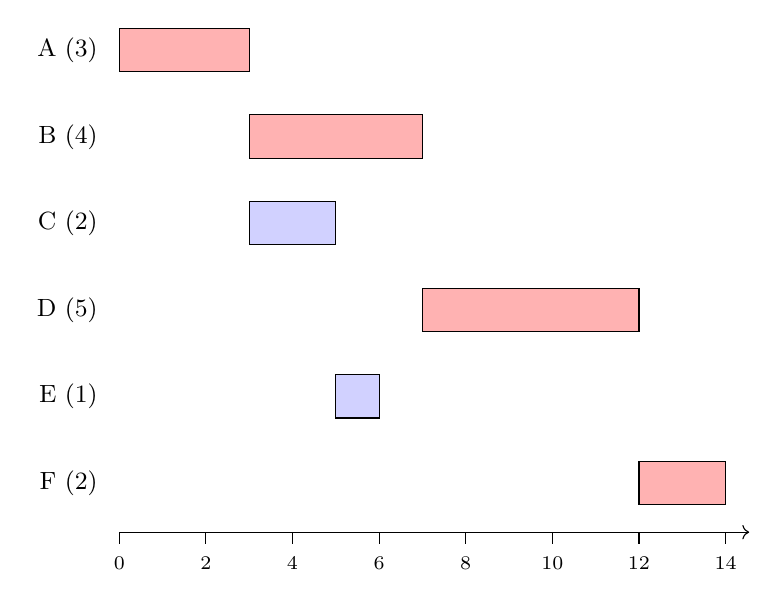
\begin{tikzpicture}[font=\small]
    \def\s{0.55}
    % ---- 活动行 ----
    \node[anchor=east] at (-0.15,5.27) {A (3)};
    \draw[fill=red!30] (0,5.0) rectangle ({3*\s},5.55);
    \node[anchor=east] at (-0.15,4.17) {B (4)};
    \draw[fill=red!30] ({3*\s},3.9) rectangle ({7*\s},4.45);
    \node[anchor=east] at (-0.15,3.07) {C (2)};
    \draw[fill=blue!18] ({3*\s},2.8) rectangle ({5*\s},3.35);
    \node[anchor=east] at (-0.15,1.97) {D (5)};
    \draw[fill=red!30] ({7*\s},1.7) rectangle ({12*\s},2.25);
    \node[anchor=east] at (-0.15,0.87) {E (1)};
    \draw[fill=blue!18] ({5*\s},0.6) rectangle ({6*\s},1.15);
    \node[anchor=east] at (-0.15,-0.23) {F (2)};
    \draw[fill=red!30] ({12*\s},-0.5) rectangle ({14*\s},0.05);
    % ---- 时间轴 ----
    \draw[->] (0,-0.85) -- ({14*\s+0.3},-0.85);
    \foreach \x in {0,2,4,6,8,10,12,14} {
        \draw (\x*\s,-0.85) -- (\x*\s,-1.0);
        \node[font=\scriptsize] at (\x*\s,-1.25) {\x};
    }
\end{tikzpicture}
\caption{项目甘特图（深色为关键活动，括号内为工期）}
\end{figure}

\subsection{PERT 与关键路径法 CPM}

\textbf{关键路径法 (CPM)} 把项目建成\textbf{活动在网络 (AON)}：节点是活动，箭头表示先后约束。对每个活动计算四个时间：

\begin{itemize}
    \item 最早开始 $ES$、最早完成 $EF = ES + \text{工期}$：沿网络\textbf{正向}推进，$ES=\max(\text{所有前置的 } EF)$。
    \item 最晚完成 $LF$、最晚开始 $LS = LF - \text{工期}$：沿网络\textbf{反向}推进，$LF=\min(\text{所有后继的 } LS)$，终点 $LF$ 取项目总工期。
\end{itemize}

\textbf{总浮动时间 (Total Float)} 为

\begin{equation}
    TF = LS - ES = LF - EF
\end{equation}

$TF=0$ 的活动组成\textbf{关键路径}，其长度等于项目最短工期；关键活动一旦延误，整个项目立即延误。示例项目活动与计算结果如下：

\begin{table}[H]
\centering
\caption{示例项目活动表与 CPM 计算结果}
\begin{tabulary}{\textwidth}{CCCCCCCC}
\toprule
活动 & 工期 & 前置 & $ES$ & $EF$ & $LS$ & $LF$ & $TF$ \\
\midrule
A & 3 & -- & 0 & 3 & 0 & 3 & 0 \\
B & 4 & A & 3 & 7 & 3 & 7 & 0 \\
C & 2 & A & 3 & 5 & 9 & 11 & 6 \\
D & 5 & B & 7 & 12 & 7 & 12 & 0 \\
E & 1 & C & 5 & 6 & 11 & 12 & 6 \\
F & 2 & D, E & 12 & 14 & 12 & 14 & 0 \\
\bottomrule
\end{tabulary}
\end{table}

\noindent 关键路径为 $A \to B \to D \to F$，工期 $3+4+5+2=14$。活动 C、E 各有 6 个时间单位的浮动，可在不影响总工期的前提下适当推迟或调配资源。

\section{风险管理}

\subsection{风险识别与评估}

\textbf{风险}是「尚未发生、但一旦发生会危害项目」的潜在事件。管理流程为：识别 $\to$ 分析（概率 $\times$ 影响）$\to$ 制定应对 $\to$ 监控。风险值用「发生概率」与「影响程度」的乘积度量：

\begin{equation}
    R = P(\text{风险}) \times I(\text{影响})
\end{equation}

\noindent 常见风险来源分四类：\textbf{技术}（技术不成熟、需求不稳）、\textbf{人员}（流失、技能不足）、\textbf{组织}（预算削减、变更失控）、\textbf{外部}（供应商、法规）。下表给出典型风险登记册：

\begin{table}[H]
\centering
\caption{风险登记册示例（概率、影响取 $1\sim5$）}
\begin{tabulary}{\textwidth}{LCCCL}
\toprule
风险 & 概率 $P$ & 影响 $I$ & $R=P\times I$ & 应对策略 \\
\midrule
需求蔓延 & 4 & 4 & 16 & 缓解：变更控制、原型确认 \\
关键技术不成熟 & 3 & 4 & 12 & 规避：技术预研、留备选 \\
核心人员流失 & 2 & 5 & 10 & 缓解：文档化、结对、备份 \\
第三方组件延误 & 3 & 3 & 9 & 转移：合同条款、多供应商 \\
预算削减 & 3 & 5 & 15 & 缓解/接受：优先级排序与储备 \\
\bottomrule
\end{tabulary}
\end{table}

\subsection{风险应对策略}

针对高 $R$ 值风险，需选择并落实应对策略：

\begin{itemize}
    \item \textbf{规避 (Avoid)}：改变计划以消除风险源，如采用成熟技术替代未验证方案。
    \item \textbf{转移 (Transfer)}：把后果转给第三方，如外包、保险、固定价合同。
    \item \textbf{缓解 (Mitigate)}：降低发生概率或影响，如增加评审、冗余设计、缓冲。
    \item \textbf{接受 (Accept)}：风险影响小或应对成本过高时，预留应急储备并监控。
\end{itemize}

\begin{table}[H]
\centering
\caption{概率--影响矩阵与处置建议}
\begin{tabulary}{\textwidth}{CCCC}
\toprule
 & 影响低 & 影响中 & 影响高 \\
\midrule
概率高 & 缓解 & 缓解/规避 & 规避/转移 \\
概率中 & 接受 & 缓解 & 规避/转移 \\
概率低 & 接受 & 接受 & 缓解/转移 \\
\bottomrule
\end{tabulary}
\end{table}

\noindent 风险管理的输出是可跟踪的\textbf{风险登记册}与\textbf{应急储备}：不仅登记风险，还要指定负责人、触发条件与应对动作，并随项目推进持续复审。

\section{软件质量}

\subsection{ISO 质量模型}

\textbf{ISO/IEC 9126}（后演化为 ISO/IEC 25010）从多个质量特性刻画软件质量，常归纳为「功能性、可靠性、易用性、效率、可维护性、可移植性」等：

\begin{table}[H]
\centering
\caption{ISO 质量特性}
\begin{tabulary}{\textwidth}{LL}
\toprule
质量特性 & 含义 \\
\midrule
功能性 (Functionality) & 满足所声明与隐含需求的能力 \\
可靠性 (Reliability) & 在规定条件下维持规定性能的能力 \\
易用性 (Usability) & 被理解、学习、使用的难易程度 \\
效率 (Efficiency) & 时间与资源利用的效率 \\
可维护性 (Maintainability) & 被修改、纠错、适应、完善的能力 \\
可移植性 (Portability) & 迁移到其他环境的能力 \\
\bottomrule
\end{tabulary}
\end{table}

\subsection{质量度量}

质量特性需用可度量的指标落地。常用度量包括：

\begin{equation}
    D = \frac{\text{缺陷总数}}{\text{KLOC}} \quad \text{(缺陷密度, defects/KLOC)}
\end{equation}
\begin{equation}
    MTBF = MTTF + MTTR
\end{equation}
\begin{equation}
    A = \frac{MTTF}{MTTF + MTTR} \quad \text{(可用度, Availability)}
\end{equation}

其中 $MTTF$ 为平均无故障时间，$MTTR$ 为平均修复时间。由公式可见：提高可用度有两条路——\textbf{降低故障率}（增大 $MTTF$）或\textbf{加快恢复}（减小 $MTTR$）。工程上常在两者间权衡，例如高可用系统用冗余提高 $MTTF$、用自动故障转移压缩 $MTTR$。

\begin{table}[H]
\centering
\caption{常用质量度量指标}
\begin{tabulary}{\textwidth}{LLL}
\toprule
指标 & 定义 & 关注点 \\
\midrule
缺陷密度 & 缺陷数 / KLOC & 开发与测试阶段的缺陷控制 \\
可靠性 & 失效概率、$MTTF$ & 长时间稳定运行能力 \\
$MTBF$ & $MTTF+MTTR$ & 平均故障间隔，可维护系统 \\
可用度 $A$ & $MTTF/MTBF$ & 服务可用的时间占比 \\
\bottomrule
\end{tabulary}
\end{table}

\noindent 度量本身不是目的：质量模型提供「看哪些维度」，度量提供「量多大」，而评审、测试与过程改进才是「把质量做出来」的手段。


\end{document}
